% English version of the IEEE article (IEEEtran, two-column journal). Translated from ../ieee/ (Spanish).
% Tables:  uv run --offline python scripts/ieee_tables.py && uv run --offline python scripts/tables_en.py
% Figures: uv run --offline python scripts/paper_figures.py --lang en --out paper/ieee_en
% Compile: pdflatex main && bibtex main && pdflatex main && pdflatex main
\documentclass[journal]{IEEEtran}

\usepackage[T1]{fontenc}
\usepackage[utf8]{inputenc}
\usepackage[english]{babel}
\usepackage{amsmath,amssymb}
\usepackage{bm}
\usepackage{cite}
\usepackage{graphicx}
\usepackage{booktabs}
\usepackage{array}
\usepackage{adjustbox}
\usepackage{makecell}
\usepackage{xcolor}
\usepackage{tikz}
\usetikzlibrary{positioning,arrows.meta}
\usepackage[hidelinks]{hyperref}

\graphicspath{{./}}
\newcommand{\var}[1]{\texttt{#1}}  % variant name (escape _ as \_)
\newcommand{\softmax}{\operatorname{softmax}}
\newcommand{\dwconv}{\operatorname{DWConv}}
\newcommand{\citep}[1]{\cite{#1}}
\newenvironment{anchocompleto}{\par\centering}{\par}
\newcommand{\anchocolumna}{\columnwidth}

\begin{document}

\title{Inductive Biases, Not Similarity Functions: A Controlled Evaluation of Performance, Scale and Calibration of Heterogeneous Attention in Small Vision Transformers}

% Sin correos: esta versión se publica como preprint en el repositorio público.
\author{Xamanek~Martínez-Marín, Jose~Adan~Hernández-Nolasco and Noel~Zacarías-Morales%
\thanks{This paper is an extended version of our paper published in Research in Computing Science 2025, 154(6), 21--33, presented as a poster at the XVII Mexican Congress of Artificial Intelligence (COMIA 2025), Universidad Panamericana, Mexico City, Mexico, 12--16 May 2025.}%
\thanks{This research was funded by the Secretaría de Ciencia, Humanidades, Tecnología e Innovación (SECIHTI, Mexico) through a graduate scholarship (Beca SECIHTI para posgrados de calidad) awarded to X.~Martínez-Marín}%
\thanks{The authors are with the División Académica de Ciencias y Tecnologías de la Información (DACYTI), Universidad Juárez Autónoma de Tabasco, Cunduacán, Tabasco, Mexico (ORCID: 0009-0008-3845-3669, 0000-0003-4671-0350 and 0000-0001-7850-6587, respectively). Corresponding author: X.~Martínez-Marín.}}

\markboth{Journal,~Vol.~X, No.~X, Month~2026}%
{Inductive Biases, Not Similarity Functions, in Small ViTs}

\maketitle

\begin{abstract}
Small Vision Transformers (ViTs) trained from scratch on limited data lack the locality bias of convolutional networks. Heterogeneous attention mechanisms (HAM), which combine two forms of attention within a head, were proposed to compensate, but were evaluated with a single run and no capacity control. We re-evaluate them in a 119k-parameter ViT and separate two families of heterogeneity: combining two similarity functions within a head, and adding to the output of each head terms with a different inductive bias, namely a depthwise convolution over the values (the LePE term of CSWin) and a global pooling summary. The protocol uses deterministic paired seeds (up to 48 per comparison), equal-capacity controls, Holm correction, four datasets (plus Food-101 for the fusions), and four published locality mechanisms for ViTs and a ResNet of the same size, all at the same parameter budget. The first family yields a well-controlled negative result: score fusions collapse onto one branch, and no similarity combination beats a capacity control (+0.15 points). In the second, a $5\times5$ depthwise convolution over the values adds, over an equal-capacity control, 5.3 points on CIFAR-10 (16 of 16 seeds), 5.4 on CIFAR-100 and 2.8 on SVHN, with 3.4\% more MACs. The gain holds with CutMix, which does not induce local heads at this scale, and from 119k to 3.6M parameters. The term matches LocalViT at lower cost and beats SPT+LSA, ConViT and a convolutional stem, although the ResNet stays 1.8 points ahead. The triad of pairwise similarity, global summary and neighborhood beats its capacity control by 0.61 points in a contrast declared before extending it to 48 seeds ($p=0.008$; $+0.67$ on the 32 new seeds, $p=0.025$) and is better calibrated, but at 1.78 times the epoch time it misses the cost criterion set in advance. Effects of half a point in this regime need tens of paired seeds to be resolved. The useful heterogeneity lies in inductive biases, not in similarity functions.
\end{abstract}

\begin{IEEEkeywords}
Vision transformers, heterogeneous attention, inductive bias, local attention, model calibration, efficient deep learning.
\end{IEEEkeywords}

% Section I: Introduction
\section{Introduction}
\label{sec:introduccion}
\IEEEPARstart{V}{ision} Transformers (ViTs) \cite{dosovitskiy2021image} reach the state of the art in image classification when pretrained at large scale, but their compact variants, trained from scratch on limited data, generalize worse than convolutional networks. CNNs build in inductive biases such as spatial locality and translation equivariance; a ViT splits the image into linearly projected patches and relies on the network to learn the spatial topology from position encodings. With enough data, attention learns local patterns in the first layers \cite{raghu2021vision}. With little data and a small model, such as the 119,290-parameter model of this work, it does not: the mean attention distance is 14 to 17 pixels on 32-pixel images in every layer.

Compact architectures are of interest when both data and compute are scarce: they must learn from small datasets, from scratch and at a low training cost. This work studies that regime (data efficiency, convergence speed and calibration). Deployment on edge devices (\emph{Edge AI}) is a further motivation, but here we only measure the inference cost on a desktop CPU; embedded hardware is not evaluated (Section~\ref{sec:res-costos}). Heterogeneous attention mechanisms (HAM), which combine more than one way of mixing the values within a head, have been proposed to improve the attention of these models. In previous work \cite{martinez2025reconfiguration} we proposed two such mechanisms for the same ViT: HAM A and HAM B, which combine in each head the output of self-attention with that of a pooling-type additive attention (\emph{soft attention}), through the Hadamard product and the element-wise sum, respectively. HAM B reached 81.07~\% accuracy on CIFAR-10, 1.3 points above the reference ViT (79.77~\%), and peaked earlier. That evaluation used a single run per variant, a constant learning rate of 0.01 and the best of 400 epochs measured on the test set; at the last epoch HAM B was below the reference (76.93 versus 79.02~\%). This work revisits those results with a controlled protocol and separates two ways of understanding heterogeneity: combining two similarity functions over the same queries and keys, or adding to the attention output terms with an inductive bias that attention lacks. The most complete configuration, which we call the \emph{triad}, brings three biases together in each head: global pairwise similarity, a global summary of the image and spatial neighborhood. The central question is how much of its gain is due to each bias and how much to the parameters it adds.

The term that turns out to matter is not new: the depthwise convolution over the values is the locally enhanced positional encoding (LePE) of CSWin \cite{dong2022cswin}. The contribution of this work is therefore not a new architecture but a controlled measurement, with three parts: a well-controlled negative result on fusing similarity functions, the contribution of each inductive bias separated from the parameters it adds, and methodological evidence on how many seeds are needed to compare attention variants in this regime.

The contributions are the following:
\begin{itemize}
  \item A controlled evaluation of two families of heterogeneous mechanisms in a small ViT: the same architecture, paired seeds with deterministic training, 16 seeds in the main comparison, equal-capacity controls and correction for multiple comparisons, on CIFAR-10, CIFAR-100, SVHN and PlantVillage, and on Food-101 for the fusions.
  \item A well-controlled negative result for the original HAM hypothesis, and its explanation: mixing scores before the \emph{softmax} multiplies the distributions, so one branch decides, and no fusion separates from a control with the same parameters.
  \item A measurement of the contribution of a local term, a depthwise convolution over the values of each head: $+5.31$ points on CIFAR-10 over an equal-capacity control ($+5.64$ over the base model), with 4.2~\% more parameters (3.1~\% of them effective) and 3.4~\% more MACs, better calibration and robustness, and 3.7 times less GPU time to reach 79~\% validation accuracy, close to the final value of the base model.
  \item A decomposition of the triad with equal-capacity controls and controls for the fusion projection: the neighborhood explains almost all of the gain; the global summary branch adds $+0.61$ points over an equal-capacity control in a contrast declared in advance and extended to 48 seeds ($+0.67$ on the 32 new seeds), and improves calibration. The triad, however, does not meet the cost criterion set in advance.
  \item A test of the scope of the local term: it holds on four datasets, with CutMix (which does not induce local heads at this scale) and from 119,000 to 3.6 million parameters, and it is compared with four published locality mechanisms for ViTs, reimplemented at the same budget, and with a ResNet of the same size.
  \item An analysis of its effects on attention and methodological evidence for this regime: the local term gives rise to two training modes, which inflate the variance of the paired differences, so half-point effects need tens of paired seeds to be resolved.
\end{itemize}

To consider that a variant works, four criteria were set in advance: a significant gain over an equal-capacity control, a balanced contribution of each branch, the same sign on another dataset and a cost of at most 1.5 times the epoch time of the base model (Section~\ref{sec:analisis}). No variant meets all four; the triad fails the cost criterion (Section~\ref{sec:res-criterios}). The rest of the article is organized as follows: Section~\ref{sec:trabajos} reviews related work; Sections~\ref{sec:metodologia} and~\ref{sec:diseno} describe the mechanisms and the experimental design; Section~\ref{sec:resultados} presents the results; Section~\ref{sec:discusion} discusses them, and Section~\ref{sec:conclusiones} concludes. The ablations of the output terms, the attention maps and a sensitivity analysis of the threshold that separates the two training modes are given as Supplementary Material.

% Section II: Related work
\section{Related Work}
\label{sec:trabajos}
CNNs dominated visual learning thanks to their biases of spatial locality and weight sharing. Self-attention \cite{vaswani2017attention} relates any two positions directly, at a cost quadratic in the number of tokens, $O(n^2 d)$, and the ViT \cite{dosovitskiy2021image} applied it to images split into $16\times16$ patches.

Three routes have been followed to make up for the lack of local biases in ViTs (Table~\ref{tab:literatura}).
\begin{itemize}
  \item \textbf{Convolution--Transformer hybrids.} LeViT \cite{graham2021levit} prepends a convolutional stage and reduces the resolution by stages. MobileViT \cite{mehta2022mobilevit} interleaves MobileNet blocks with blocks that combine convolutions and attention over unfolded patches. CMT \cite{guo2022cmt} interleaves convolutional blocks. CvT \cite{wu2021cvt} uses convolutions in the token embedding and in the query, key and value projections of each stage.
  \item \textbf{Attention restricted to windows.} Swin \cite{liu2021swin} computes attention within local $M\times M$ windows, at a cost of $O(N M^2 d)$, and shifts them between layers to connect them; no layer has a direct global interaction.
  \item \textbf{Convolutions injected into attention, position or the MLP.}
  \begin{itemize}
    \item ConViT \cite{dascoli2021convit} initializes attention as a convolution, with a learned gate that weighs the positional part against the content part.
    \item CSWin \cite{dong2022cswin} adds a depthwise convolution over the values to the attention output (LePE).
    \item Conditional position encodings \cite{chu2023conditional} generate the position with a convolution.
    \item LocalViT \cite{li2021localvit} inserts a depthwise convolution into the feed-forward network.
  \end{itemize}
\end{itemize}
For small datasets, Lee \emph{et al.} \cite{lee2021vision} propose tokenizing with shifted patches (SPT) and learning the attention temperature while masking the diagonal (LSA), and Xiao \emph{et al.} \cite{xiao2021early} show that replacing the patch projection with a convolutional stem stabilizes training. These architectures were designed and evaluated at scales of millions of parameters (28 to 88 million in Swin) and change several components at once. Section~\ref{sec:res-baselines} reimplements four of them (LocalViT, SPT+LSA, ConViT and the convolutional stem), together with a ResNet, with the budget and protocol of this work.

Locality can also come from the data. CutMix \cite{yun2019cutmix}, Mixup \cite{zhang2018mixup} and RandAugment \cite{cubuk2020randaugment} are a standard part of training ViTs on little data, and Santiago Toledo and Martínez \cite{santiago2026inducing} found that CutMix, unlike other augmentations, suffices for a 2.4-million-parameter ViT to develop local heads. If that happened at any scale, an architectural neighborhood bias would be redundant with the training protocol; Section~\ref{sec:res-aumento} puts this to the test.

Among attention mechanisms, additive attention \cite{bahdanau2015neural} is the classic alternative to the dot product, and the multiplicative gate after attention improves the stability of large language models \cite{qiu2025gated}. Reading attention weights as explanations is debated \cite{jain2019attention}; \emph{attention rollout} \cite{abnar2020quantifying} propagates them through the layers. The idea of combining two similarity functions within a head comes from the preliminary results that motivated this study (Section~\ref{sec:introduccion}). Here we show that mixing their scores before the \emph{softmax} amounts to multiplying the distributions of each branch (Section~\ref{sec:metodologia}).

Compared with these works, the triad evaluated here:
\begin{itemize}
  \item keeps global dot-product attention in every layer, unlike Swin;
  \item does not change the projections or the resolution, unlike CvT, LeViT or MobileViT;
  \item adds the local bias as a zero-initialized residual term, the same as LePE, and a global summary combined after the \emph{softmax}.
\end{itemize}
Its goal is not to propose an architecture, but to measure how much each bias contributes on its own in a 119,290-parameter ViT trained from scratch, with capacity controls.

\begin{table*}[!t]
\centering
\small
\caption{Properties of representative architectures compared with the variants evaluated in this work.}
\label{tab:literatura}
\begin{anchocompleto}
\begin{tabular}{>{\raggedright\arraybackslash}p{2.6cm}>{\raggedright\arraybackslash}p{3.4cm}>{\raggedright\arraybackslash}p{3.6cm}>{\raggedright\arraybackslash}p{2.8cm}>{\raggedright\arraybackslash}p{3.6cm}}
\toprule
Architecture & Attention mechanism & Local bias & Complexity & Main limitations \\
\midrule
ViT \cite{dosovitskiy2021image} & Scaled dot product ($\mathbf{Q}\mathbf{K}^\top/\sqrt{d}$) & None (position encoding only) & $O(N^2 d)$ & Needs large-scale pretraining; with little data it generalizes worse than a CNN. \\
Swin \cite{liu2021swin} & Shifted-window attention & Local windows and relative position bias & $O(N M^2 d)$ & No direct global interactions within a single layer. \\
CvT \cite{wu2021cvt} & Dot product with convolutional projections & Convolutions in the $\mathbf{Q},\mathbf{K},\mathbf{V}$ projections & $O(N^2 d) + O(N k^2 d)$ & Changes the projections of every layer. \\
LeViT \cite{graham2021levit} & Dot product with positional attention bias & Initial convolutional stage and stage-wise resolution reduction & $O(N^2 d)$ per stage, on reduced grids & Changes the whole architecture; designed for fast inference. \\
MobileViT \cite{mehta2022mobilevit} & Dot product over unfolded patches & MobileNet blocks and convolutions within each block & $O(P N^2 d)$, with $P$ pixels per patch & Designed for mobile devices; mixes convolution and attention in every block. \\
CSWin / LePE \cite{dong2022cswin} & Cross-shaped window attention & Depthwise convolution over $\mathbf{V}$ added to the output & $O(N\sqrt{N} d) + O(N k^2 d)$ & Evaluated only together with cross-shaped window attention. \\
LocalViT \cite{li2021localvit} & Scaled dot product & Depthwise convolution in the feed-forward network & $O(N^2 d) + O(N k^2 d)$ & The local bias is in the MLP, not in the attention output. \\
This work (triad) & \var{dot}, global summary (additive \emph{pooling}) and concatenation (\var{ham\_concat}) & Depthwise $k\times k$ convolution over $\mathbf{V}$ in each head (LePE) & $O(N^2 d) + O(N k^2 d)$ & Costs 1.78 times the epoch time of \var{dot}, mostly because of the \emph{pooling} branch with the concatenation (1.68 times on its own). \\
\bottomrule
\end{tabular}
\end{anchocompleto}
\end{table*}

% Section III: Methodology
\section{Methodology}
\label{sec:metodologia}

\subsection{Vision Transformer Architecture}
\label{sec:vit}

\subsubsection{Overview}
All experiments use the same small pre-norm Vision Transformer (ViT) \citep{dosovitskiy2021image}: hidden dimension $D=48$, $L=4$ blocks, $H=4$ heads of dimension $d=D/H=12$, a multilayer perceptron (MLP) with a 192-unit hidden layer and GELU activation \citep{hendrycks2016gelu}, and a dropout of 0.1 on the projections, the MLP, the residual connections and the attention weights. With these dimensions the base model has 119,290 parameters. Each block computes
\begin{align}
  \mathbf{X}' &= \mathbf{X} + \operatorname{MHA}\big(\operatorname{LN}(\mathbf{X})\big), \\
  \mathbf{X}'' &= \mathbf{X}' + \operatorname{MLP}\big(\operatorname{LN}(\mathbf{X}')\big),
\end{align}
with $\operatorname{LN}$ layer normalization \citep{ba2016layer}. Classification uses a linear layer on the class token (CLS) of the last layer, after a final normalization. A model of this size was chosen so that each variant could be trained with many seeds and the full protocol (Section~\ref{sec:entrenamiento}); the price is that the results refer to small ViTs trained from scratch on small datasets.

\subsubsection{Image Representation as Tokens}
An $S\times S$-pixel image is split into $P\times P$ patches, which are projected to dimension $D$ with a stride-$P$ convolution. A learned CLS token is prepended and a learned position encoding is added, so the sequence has $N = 1 + (S/P)^2$ tokens. On CIFAR-10 ($S=32$, $P=4$) the patches form an $8\times8$ grid and $N=65$; on PlantVillage ($S=64$, $P=4$), a $16\times16$ grid and $N=257$.

\subsubsection{Self-Attention Mechanism}
Each head $h$ projects the normalized input $\mathbf{X}\in\mathbb{R}^{N\times D}$ to queries, keys and values $\mathbf{Q}_h,\mathbf{K}_h,\mathbf{V}_h\in\mathbb{R}^{N\times d}$ with a single shared linear projection $\mathbf{W}_{qkv}$. Scaled dot-product attention \citep{vaswani2017attention}, which we call \var{dot}, is
\begin{equation}
  \mathbf{A}_h = \softmax\!\left(\frac{\mathbf{Q}_h\mathbf{K}_h^\top}{\sqrt{d}}\right), \qquad
  \mathbf{O}_h = \mathbf{A}_h \mathbf{V}_h,
  \label{eq:dot}
\end{equation}
with the \emph{softmax} taken row-wise: row $i$ of $\mathbf{A}_h$ is the distribution with which token $i$ combines the values of all tokens. The head outputs are concatenated and passed through an output projection, $\operatorname{MHA}(\mathbf{X}) = [\mathbf{O}_1\Vert\cdots\Vert\mathbf{O}_H]\,\mathbf{W}_o$.

\subsection{Heterogeneous Attention Mechanisms}
\label{sec:ham}
A heterogeneous attention mechanism (HAM) combines, within a head, more than one way of mixing the values. Two families were studied: the combination of two attention functions over the same $\mathbf{Q}_h,\mathbf{K}_h,\mathbf{V}_h$ (Section~\ref{sec:fusiones}), which is the original HAM formulation, and the addition of terms with complementary inductive biases to the head output (Section~\ref{sec:terminos}). To simplify notation, the index $h$ is omitted.

\subsubsection{Attention Branches}
Besides \var{dot}, three variants of additive attention were used:
\begin{itemize}
  \item \textbf{Pooling-type additive} (\var{additive}). One score per token, $s_j = \mathbf{w}^\top\tanh(\mathbf{W}_q\mathbf{q}_j + \mathbf{W}_k\mathbf{k}_j) + b$, a single context vector $\mathbf{c} = \sum_j \softmax(\mathbf{s})_j\,\mathbf{v}_j$, and the same output $\mathbf{c}$ for every token. It does not compare pairs of tokens: it is a global summary of the image, with $O(Nd)$ memory.
  \item \textbf{Pairwise additive} (Bahdanau \citep{bahdanau2015neural}). $e_{ij} = \mathbf{w}^\top\tanh(\mathbf{W}_q\mathbf{q}_i + \mathbf{W}_k\mathbf{k}_j)$ and $\mathbf{A}=\softmax(\mathbf{E})$.
  \item \textbf{Free additive} (\var{additive\_free}). The pairwise version without its own parameters, $e_{ij} = \sum_{c=1}^{d}\tanh(q_{ic} + k_{jc})$, and its variant scaled by $1/\sqrt{d}$. Unlike \eqref{eq:dot}, it cannot be written as a matrix product and materializes an $N\times N\times d$ tensor per head.
\end{itemize}

\subsubsection{Two-Branch Fusions}
\label{sec:fusiones}
Let $\mathbf{S}_1,\mathbf{S}_2$ be the pre-\emph{softmax} scores of two pairwise branches and $\mathbf{A}_b=\softmax(\mathbf{S}_b)$. Three levels of fusion were evaluated:
\begin{itemize}
  \item \textbf{Concatenation} (\var{concat\_linear}): $\mathbf{O} = [\mathbf{A}_1\mathbf{V}\,\Vert\,\mathbf{A}_2\mathbf{V}]\,\mathbf{W}_f + \mathbf{b}_f$, with $\mathbf{W}_f\in\mathbb{R}^{2d\times d}$ per head. It also admits the \emph{pooling} branch; the combination \var{dot} + \var{additive} is \var{ham\_concat}.
  \item \textbf{Score mixing}: $\mathbf{O}=\softmax\big(\lambda\mathbf{S}_1 + (1-\lambda)\mathbf{S}_2\big)\mathbf{V}$, with $\lambda$ fixed (\var{ham\_weighted}, $\lambda=0.85$), learned per head (\var{ham\_weighted\_learn}) or with the sum $\mathbf{S}_1+\mathbf{S}_2$ (\var{ham\_sum}). Since $\softmax(\lambda\mathbf{S}_1 + (1-\lambda)\mathbf{S}_2) \propto \mathbf{A}_1^{\lambda}\odot\mathbf{A}_2^{1-\lambda}$ row by row, this fusion is a \emph{product} of distributions. A version with row-standardized scores and a learned scale per branch (\var{ham\_zscore}) was also tested.
  \item \textbf{Output mixing}: $\mathbf{O} = \lambda\,\mathbf{A}_1\mathbf{V} + (1-\lambda)\,\mathbf{A}_2\mathbf{V} = \big(\lambda\mathbf{A}_1 + (1-\lambda)\mathbf{A}_2\big)\mathbf{V}$, a mixture of distributions after the \emph{softmax}, with $\lambda$ learned (\var{ham\_wout}, \var{ham\_weighted\_learn\_out}) or with a per-token gate $\mathbf{g}_i = \softmax(\mathbf{W}_g[\mathbf{o}_{1i}\Vert\mathbf{o}_{2i}])$ (\var{ham\_gated}).
\end{itemize}
Finally, \var{ham\_heads} assigns different branches to different heads (two \var{dot} and two \emph{pooling}), with no fusion within the head.

\subsubsection{Output Terms with Complementary Inductive Biases}
\label{sec:terminos}
The second family does not add another similarity function: it adds to the output of each head, before $\mathbf{W}_o$, terms that bring information that pairwise attention does not have.
\begin{itemize}
  \item \textbf{Local term} (\var{local}). A $k\times k$ channel-separable (depthwise) convolution over the values, arranged on the patch grid:
  \begin{equation}
    \mathbf{O} \leftarrow \mathbf{O} + \dwconv_{k\times k}\big(\mathbf{V}_{\text{patches}}\big),
    \label{eq:local}
  \end{equation}
  with an independent filter for each channel of each head ($Hd$ groups) and padding that preserves the grid size; the CLS receives 0. It is the locally-enhanced positional encoding (LePE) of CSWin \citep{dong2022cswin}. It costs $Hd(k^2+1)$ parameters per layer: 480 with $k=3$ and 1,248 with $k=5$.
  \item \textbf{Gate} (\var{gate}): $\mathbf{O}\leftarrow\mathbf{O}\odot 2\sigma(\mathbf{X}\mathbf{W}_g + \mathbf{b}_g)$ per token, head and channel, as in \emph{Gated Attention} \citep{qiu2025gated}. It introduces a nonlinearity between $\mathbf{W}_v$ and $\mathbf{W}_o$, which would otherwise compose into a single linear map.
  \item \textbf{Residual global context} (\var{global}): $\mathbf{O}\leftarrow\mathbf{O} + \bm{\alpha}\odot\mathbf{c}$, with $\mathbf{c}$ the context of the \emph{pooling} branch and $\bm{\alpha}\in\mathbb{R}^{d}$ a per-channel scale.
\end{itemize}
The three terms start at the identity (convolution weights and $\bm{\alpha}$ at zero; gate equal to 1) and are initialized with a separate random generator. Consequently, with the same seed, a model with output terms starts with exactly the same weights and the same outputs as \var{dot}, and any difference is due to what it learns. The terms are applied after the fusion, so they are compatible with any branch or fusion. The most complete model, \var{ham\_concat\_local\_k5}, computes in each head
\begin{equation}
  \mathbf{O} = \big[\mathbf{A}^{\text{dot}}\mathbf{V}\,\Vert\,\mathbf{1}\mathbf{c}^\top\big]\,\mathbf{W}_f + \mathbf{b}_f + \dwconv_{5\times5}(\mathbf{V}_{\text{patches}}),
  \label{eq:final}
\end{equation}
that is, it combines three inductive biases in each head, each in its own term: global pairwise similarity ($\mathbf{A}^{\text{dot}}\mathbf{V}$), a global summary of the image ($\mathbf{1}\mathbf{c}^\top$) and spatial neighborhood ($\dwconv_{5\times5}$). From here on we call it the \emph{triad}. Fig.~\ref{fig:triada} shows its place in the encoder block. The two attention branches are combined after the \emph{softmax}, and the local term is added outside the fusion, so none of the three biases can cancel another, as happens when scores are mixed.

\begin{figure*}[!t]
\begin{anchocompleto}
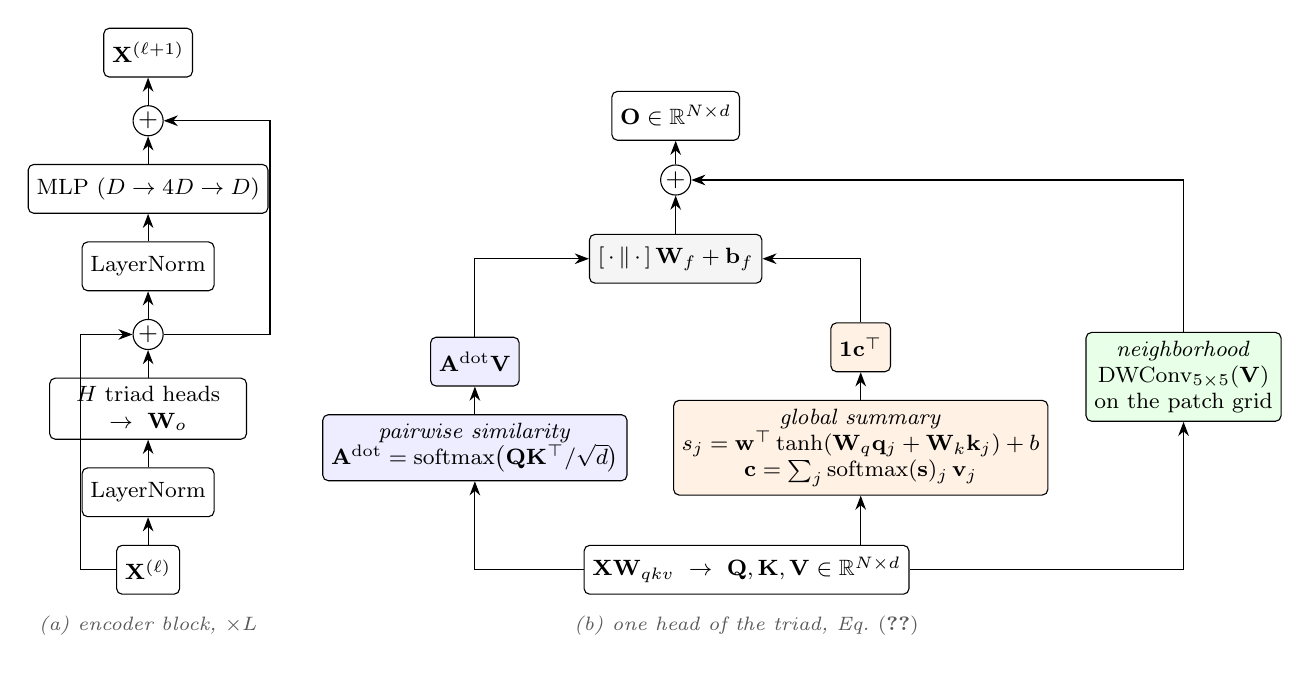
\begin{tikzpicture}[
  font=\footnotesize, >={Stealth[length=1.8mm]},
  op/.style={draw, rounded corners=2pt, align=center, inner sep=3pt, minimum height=0.62cm, fill=white},
  dot/.style={op, fill=blue!7}, glob/.style={op, fill=orange!10}, loc/.style={op, fill=green!9},
  sum/.style={draw, circle, inner sep=0.5pt, font=\small},
  lab/.style={font=\scriptsize\itshape, text=black!65}]
  % (a) encoder block
  \node[op] (x) at (0,0) {$\mathbf{X}^{(\ell)}$};
  \node[op, above=0.35cm of x] (ln1) {LayerNorm};
  \node[op, above=0.35cm of ln1, minimum width=2.5cm] (mha) {$H$ triad heads\\$\to\ \mathbf{W}_o$};
  \node[sum, above=0.35cm of mha] (r1) {$+$};
  \node[op, above=0.35cm of r1] (ln2) {LayerNorm};
  \node[op, above=0.35cm of ln2] (mlp) {MLP ($D\to4D\to D$)};
  \node[sum, above=0.35cm of mlp] (r2) {$+$};
  \node[op, above=0.35cm of r2] (y) {$\mathbf{X}^{(\ell+1)}$};
  \foreach \a/\b in {x/ln1, ln1/mha, mha/r1, r1/ln2, ln2/mlp, mlp/r2, r2/y} \draw[->] (\a) -- (\b);
  \draw[->] (x.west) -- ++(-0.45,0) |- (r1.west);
  \draw[->] (r1.east) -- ++(1.35,0) |- (r2.east);
  \node[lab, below=0.15cm of x] {(a) encoder block, $\times L$};
  % (b) one head of the triad
  \begin{scope}[xshift=7.6cm]
    \node[op] (in) at (0,0) {$\mathbf{X}\mathbf{W}_{qkv}\ \to\ \mathbf{Q},\mathbf{K},\mathbf{V}\in\mathbb{R}^{N\times d}$};
    \node[dot] (att) at (-3.45,1.55) {\textit{pairwise similarity}\\$\mathbf{A}^{\text{dot}}=\softmax\!\big(\mathbf{Q}\mathbf{K}^\top/\sqrt{d}\big)$};
    \node[dot, above=0.35cm of att] (av) {$\mathbf{A}^{\text{dot}}\mathbf{V}$};
    \node[glob] (pool) at (1.45,1.55) {\textit{global summary}\\$s_j=\mathbf{w}^\top\tanh(\mathbf{W}_q\mathbf{q}_j+\mathbf{W}_k\mathbf{k}_j)+b$\\$\mathbf{c}=\sum_j\softmax(\mathbf{s})_j\,\mathbf{v}_j$};
    \node[glob, above=0.35cm of pool] (bc) {$\mathbf{1}\mathbf{c}^\top$};
    \node[op, fill=black!4] (fus) at (-0.9,3.95) {$[\,\cdot\,\Vert\,\cdot\,]\,\mathbf{W}_f+\mathbf{b}_f$};
    \node[loc] (dw) at (5.55,2.45) {\textit{neighborhood}\\$\dwconv_{5\times5}(\mathbf{V})$\\on the patch grid};
    \node[sum] (s) at (-0.9,4.95) {$+$};
    \node[op, above=0.3cm of s] (o) {$\mathbf{O}\in\mathbb{R}^{N\times d}$};
    \draw[->] (in.west) -| (att.south);
    \draw[->] (in.north -| pool) -- (pool);
    \draw[->] (in.east) -| (dw.south);
    \draw[->] (att) -- (av); \draw[->] (pool) -- (bc);
    \draw[->] (av.north) |- (fus.west); \draw[->] (bc.north) |- (fus.east);
    \draw[->] (fus) -- (s); \draw[->] (dw.north) |- (s.east); \draw[->] (s) -- (o);
    \node[lab, below=0.15cm of in] {(b) one head of the triad, Eq.~\eqref{eq:final}};
  \end{scope}
\end{tikzpicture}
\end{anchocompleto}
\caption{Evaluated architecture. (a) Pre-norm ViT block. (b) Each head of the triad \var{ham\_concat\_local\_k5} combines three biases in separate terms: dot-product attention (pairwise similarity), the additive \emph{pooling} branch (a single summary $\mathbf{c}$ replicated to the $N$ tokens), both fused after the \emph{softmax} by concatenation and projection, and a $5\times5$ depthwise convolution over the patch values, added outside the fusion and initialized at zero (the CLS receives 0). Without the \emph{pooling} branch and the fusion it is \var{dot\_local\_k5}; without the local term it is \var{ham\_concat}; without both, \var{dot}.}
\label{fig:triada}
\end{figure*}

In the last layer only the CLS reaches the loss, and the local term does not act on the CLS; therefore the convolution of layer 4 receives no gradient and stays at zero. The local term is effective in layers 1 to 3: of its 4,992 parameters, 3,744 (3.1~\% of \var{dot}) are effective, and removing it from layer 4 would give the same model with 1,248 fewer parameters.

Table~\ref{tab:parametros} breaks down the parameters of the four main architectures, counted on the built model: the \emph{pooling} branch adds 4,816, the fusion 4,800 and the $5\times5$ local term 4,992, for a total of 133,898 in \var{ham\_concat\_local\_k5}, 12.2~\% more than \var{dot} (132,650 and 11.2~\% counting only the effective parameters).

% Translated by scripts/tables_en.py from the Spanish table generated by scripts/ieee_tables.py a partir de los runs; no editar a mano.

\begin{table*}[!t]
\centering
\footnotesize
\caption{Parameter budget by component, counted on the built model (4 layers, $D=48$, $H=4$, MLP 192, CIFAR-10). The \emph{pooling} branch has $\mathbf{W}_q,\mathbf{W}_k\in\mathbb{R}^{d\times d}$ and $\mathbf{w},b$ per head (301 per head); $\mathbf{W}_f\in\mathbb{R}^{2d\times d}$ with bias (300 per head); the local term, $Hd(k^2+1)=1\,248$ per layer. Effective total: without the local term of layer 4, which receives no gradient because only the CLS reaches the loss (Section~\ref{sec:terminos}).}
\label{tab:parametros}
\begin{adjustbox}{max width=\linewidth}
\begin{tabular}{lrrrr}
\toprule
Component & \texttt{dot} & \texttt{ham\_concat} & \texttt{dot\_local\_k5} & \texttt{ham\_concat\_local\_k5} \\
\midrule
Embeddings (patches, position, CLS) & 5\,520 & 5\,520 & 5\,520 & 5\,520 \\
Projection $\mathbf{Q},\mathbf{K},\mathbf{V}$ & 28\,224 & 28\,224 & 28\,224 & 28\,224 \\
Additive \emph{pooling} branch & --- & 4\,816 & --- & 4\,816 \\
Fusion $\mathbf{W}_f$ (\texttt{concat\_linear}) & --- & 4\,800 & --- & 4\,800 \\
Output projection $\mathbf{W}_o$ & 9\,408 & 9\,408 & 9\,408 & 9\,408 \\
Local term ($\dwconv_{5\times5}$) & --- & --- & 4\,992 & 4\,992 \\
MLP & 74\,688 & 74\,688 & 74\,688 & 74\,688 \\
Layer normalizations & 960 & 960 & 960 & 960 \\
Classifier & 490 & 490 & 490 & 490 \\
\midrule
Total & 119\,290 & 128\,906 & 124\,282 & 133\,898 \\
Effective total & 119\,290 & 128\,906 & 123\,034 & 132\,650 \\
\bottomrule
\end{tabular}
\end{adjustbox}
\end{table*}


% Section IV: Experimental design
\section{Experimental Design}
\label{sec:diseno}

\subsection{Datasets}
\begin{itemize}
  \item \textbf{CIFAR-10} \citep{krizhevsky2009learning}: 10 classes, $32\times32$ images. From the official training set (50,000 images), 5,000 are held out for validation with a fixed split; the model is trained on the remaining 45,000 and evaluated on the official test set (10,000 images). It is the main dataset of the study.
  \item \textbf{PlantVillage} \citep{hughes2015plantvillage}: 38 classes of healthy and diseased leaves, resized to $64\times64$. From the distributed training folder (43,444 images), 4,344 are held out for validation; the distributed validation folder (10,861 images) is used as the test set.
  \item \textbf{CIFAR-100} \citep{krizhevsky2009learning} and \textbf{SVHN} \citep{netzer2011reading}: 100 classes and 10 digits, $32\times32$ images, with 10~\% of the official training set as validation (5,000 and 7,326 images) and the official test set (10,000 and 26,032). They were used in the scope experiments (Section~\ref{sec:res-alcance}).
  \item \textbf{Food-101} \citep{bossard2014food}: 101 classes, images resized to $192\times192$ with patches of 8 ($N=577$); 75,750 official training images (10~\% for validation) and 25,250 test images. It was used only for the fusions of the first family.
\end{itemize}
Images are normalized with the per-channel mean and standard deviation of each dataset (those of ImageNet for PlantVillage and Food-101). Data augmentation is a random crop with 4-pixel padding and a horizontal flip, with no rescaling. To measure the dependence on data augmentation, a subset was repeated on CIFAR-10 without augmentation, and the key variants with two stronger protocols (Section~\ref{sec:diseno-alcance}).

\subsection{Base Architecture and Variants}
Table~\ref{tab:variantes} lists the CIFAR-10 variants with their parameters and their cost per epoch. Three controls were included:
\begin{itemize}
  \item \var{dot\_wide}: \var{dot} with the MLP hidden layer widened from 192 to 217 units, to match the parameters of \var{ham\_concat} (128,990 versus 128,906). It separates the effect of the extra branch from that of having more parameters.
  \item \var{dot\_local\_k1}: the local term~\eqref{eq:local} with $k=1$, which keeps the extra path from the values to the output but does not mix neighboring patches. It separates the effect of the neighborhood from that of the architecture of the term.
  \item \var{dot\_wide\_local\_k5}: the $5\times5$ local term on top of \var{dot\_wide}, with almost the same parameters as \var{ham\_concat\_local\_k5} (133,982 versus 133,898).
\end{itemize}

% Translated by scripts/tables_en.py from the Spanish table generated by scripts/ieee_tables.py a partir de los runs; no editar a mano.

\begin{table*}[!t]
\centering
\footnotesize
\caption{Variants evaluated on CIFAR-10. Total model parameters and training seconds per epoch (mean over seeds 0--4, RTX 5080, no other processes on the GPU).}
\label{tab:variantes}
\begin{adjustbox}{max width=\linewidth}
\begin{tabular}{llllrr}
\toprule
Variant & Branches per head & Fusion & Local term & Parameters & s/epoch \\
\midrule
\texttt{dot} & dot & --- & --- & 119\,290 & 1.38 \\
\texttt{dot\_wide} & dot (MLP 217) & --- & --- & 128\,990 & 1.41 \\
\texttt{additive} & additive \emph{pooling} & --- & --- & 124\,106 & 1.59 \\
\midrule
\texttt{ham\_concat} & dot + additive \emph{pooling} & concat & --- & 128\,906 & 2.31 \\
\texttt{ham\_pairwise} & dot + pairwise additive & concat & --- & 128\,890 & 4.00 \\
\texttt{ham\_weighted} & dot + free additive & scores, $\lambda=0.85$ & --- & 119\,290 & 2.61 \\
\texttt{ham\_weighted\_learn} & dot + free additive & scores, $\lambda$ learned & --- & 119\,306 & 2.93 \\
\texttt{ham\_sum} & dot + free additive & scores, sum & --- & 119\,290 & 2.69 \\
\texttt{ham\_zscore} & dot + free additive & standardized scores & --- & 119\,338 & 3.29 \\
\texttt{ham\_wout} & dot + additive \emph{pooling} & outputs, $\lambda$ learned & --- & 124\,122 & 2.37 \\
\texttt{ham\_gated} & dot + additive \emph{pooling} & outputs, gate & --- & 124\,906 & 2.55 \\
\texttt{ham\_weighted\_learn\_out} & dot + free additive & outputs, $\lambda$ learned & --- & 119\,306 & 2.91 \\
\texttt{ham\_heads} & 2 dot, 2 additive \emph{pooling} & across heads & --- & 121\,698 & 1.50 \\
\midrule
\texttt{dot\_local\_k1} & dot & --- & $1\times1$ & 119\,674 & 1.51 \\
\texttt{dot\_local} & dot & --- & $3\times3$ & 121\,210 & 1.47 \\
\texttt{dot\_local\_k5} & dot & --- & $5\times5$ & 124\,282 & 1.49 \\
\texttt{dot\_local\_k7} & dot & --- & $7\times7$ & 128\,890 & 1.66 \\
\texttt{dot\_gate} & dot & + gate & --- & 128\,698 & 1.44 \\
\texttt{dot\_global} & dot & + global context & --- & 124\,298 & 2.14 \\
\texttt{dot\_wide\_local\_k5} & dot (MLP 217) & --- & $5\times5$ & 133\,982 & 1.52 \\
\texttt{ham\_concat\_local} & dot + additive \emph{pooling} & concat & $3\times3$ & 130\,826 & 2.45 \\
\texttt{ham\_concat\_local\_k5} & dot + additive \emph{pooling} & concat & $5\times5$ & 133\,898 & 2.46 \\
\bottomrule
\end{tabular}
\end{adjustbox}
\par\smallskip\parbox{\linewidth}{\footnotesize concat: \texttt{concat\_linear}. scores: mixing before the \emph{softmax}; outputs: convex mixture of $A_b v$ after the \emph{softmax}. Free additive: $e_{ij}=\sum_d \tanh(q_i+k_j)_d$. Names: \texttt{\_wide}, MLP of 217 (equal-capacity control); \texttt{\_local}, $3\times3$ local term, and \texttt{\_local\_k}$k$, $k\times k$. \texttt{ham\_concat\_local\_k5} is the triad and \texttt{dot\_wide\_local\_k5} its equal-capacity control.}
\end{table*}


\subsection{Training Parameters}
\label{sec:entrenamiento}
All variants share the same hyperparameters, with no per-variant search: AdamW \citep{loshchilov2019decoupled} with a learning rate of $10^{-3}$ and a weight decay of 0.05 (except for $\lambda$, the scales of the standardized fusion and $\bm{\alpha}$), a cosine schedule \citep{loshchilov2017sgdr} with 10 epochs of linear warmup, cross-entropy without label smoothing and single precision. On CIFAR-10 training lasts 400 epochs with batches of 256; on PlantVillage, 50 epochs with batches of 128 (the largest size at which the pairwise branches fit in 16~GB); on Food-101, 50 epochs with batches of 128. The model from the epoch with the best validation accuracy is kept and the test set is evaluated only once, on that model. Table~\ref{tab:hiperparametros} gathers all hyperparameters.

\begin{table}[!t]
\centering
\footnotesize
\caption{Hyperparameters, common to all variants unless stated otherwise.}
\label{tab:hiperparametros}
\begin{tabular}{>{\raggedright\arraybackslash}p{2.6cm}>{\raggedright\arraybackslash}p{5.3cm}}
\toprule
Hyperparameter & Value \\
\midrule
\multicolumn{2}{l}{\textit{Model}} \\
Image, patch, tokens & $32\times32$, $4\times4$, $N=65$ (CIFAR, SVHN); $64\times64$, $4\times4$, $N=257$ (PlantVillage); $192\times192$, $8\times8$, $N=577$ (Food-101) \\
$D$, $L$, $H$, $d$ & 48, 4, 4, 12 \\
MLP & 192 (217 in the capacity controls), GELU (tanh approximation) \\
Normalization & LayerNorm before each sublayer, $\epsilon=10^{-6}$ \\
Dropout & 0.1 on embedding, attention, projection, MLP and residuals \\
Initialization & CLS and positions truncated $\mathcal{N}(0, 0.02)$; local term at zero; the rest, PyTorch default \\
\midrule
\multicolumn{2}{l}{\textit{Optimization}} \\
Optimizer & AdamW, $\beta=(0.9, 0.999)$, $\epsilon=10^{-8}$ \\
Learning rate & $10^{-3}$, cosine with 10 epochs of linear warmup \\
Weight decay & 0.05 (0 on $\lambda$, fusion scales and $\bm{\alpha}$) \\
Batch, epochs & 256, 400 (CIFAR-10 and CIFAR-100); 256, 100 (SVHN); 128, 50 (PlantVillage and Food-101) \\
Loss & cross-entropy, no label smoothing \\
Data augmentation & crop with 4-pixel padding and horizontal flip (no flip on SVHN) \\
Precision & FP32, deterministic algorithms \\
\midrule
\multicolumn{2}{l}{\textit{Evaluation}} \\
Selection & best validation accuracy; test evaluated once \\
Seeds & 0--4; 0--15 in the main comparison; 0--47 in the primary contrast \\
\midrule
\multicolumn{2}{l}{\textit{Augmentation arms (Section~\ref{sec:res-aumento})}} \\
CutMix & $\alpha=1$, probability 0.6 \\
Strong augmentation & RandAugment (2 operations, magnitude 9), CutMix or Mixup ($\alpha=1$) on each batch, label smoothing 0.1 \\
\bottomrule
\end{tabular}
\end{table}

Each variant was trained with 5 seeds (0 to 4). The variants of the main comparison were later extended to 16 seeds (0 to 15). The seed fixes the initialization, the batch order, the data augmentation and the dropout masks; the training/validation split is the same for all. Training is deterministic: with the same code and the same seed the metrics are reproduced bit for bit, which allows comparisons to be paired by seed across experiments run at different times. Each run records the code commit. An NVIDIA RTX 5080 GPU was used with PyTorch 2.14 and CUDA 13.0, one run at a time.

\subsection{Scope Experiments}
\label{sec:diseno-alcance}
For Section~\ref{sec:res-alcance}, four published locality mechanisms for ViTs and a ResNet of the same size were implemented with the same parameter budget as the variants of this work and without changing the hyperparameters of Table~\ref{tab:hiperparametros}:
\begin{itemize}
  \item \textbf{LocalViT} \citep{li2021localvit}: a $3\times3$ depthwise convolution and an activation between the two MLP layers, on the patch tokens (126,970 parameters).
  \item \textbf{SPT+LSA} \citep{lee2021vision}: tokenization with the image shifted by half a patch along the four diagonals, and attention with a learned temperature and a masked diagonal (129,002).
  \item \textbf{ConViT} \citep{dascoli2021convit}: attention with a gate between content and relative position, with the positional part initialized as a convolution, in all four layers; an MLP of 205 to match parameters (124,398).
  \item \textbf{Convolutional stem} \citep{xiao2021early}: two stride-2 $3\times3$ convolutions with batch normalization and ReLU, and one $1\times1$ convolution, instead of the patch projection (130,450).
  \item \textbf{ResNet} \citep{he2016deep}: three stages of one basic block, with 20, 40 and 80 channels (121,390).
\end{itemize}
The five key variants (\var{dot}, \var{dot\_wide}, \var{dot\_local\_k5}, \var{dot\_wide\_local\_k5} and the triad) were repeated with two additional augmentation protocols (Table~\ref{tab:hiperparametros}), on CIFAR-100 and SVHN, and with 10, 25 and 50~\% of the CIFAR-10 training set (\var{dot\_wide} was not run with fractions). The fractions are a fixed subset, the same for all seeds. For model size, $D$ and $L$ were varied with 4 heads and an MLP of $4D$, and only \var{dot} and \var{dot\_local\_k5} were compared, with seeds 0 to 2. The resulting sizes of \var{dot} are 119,290, 232,378, 459,754, 907,114, 1,804,234 and 3,583,690 parameters.

\subsection{Attention and Model Analysis}
\label{sec:analisis}
\subsubsection{Statistics} For each pair of variants, the per-seed difference in test accuracy, $\Delta_s$, is computed, and we report its mean with a Student's $t$ 95~\% confidence interval (CI), the number of seeds with $\Delta_s>0$, the $p$-value of the paired $t$-test and, with 16 seeds, that of the Wilcoxon signed-rank test \citep{wilcoxon1945individual}. Within each table, multiple comparisons are corrected with the Holm method \citep{holm1979simple}, which is step-down: with $m$ comparisons, the $i$-th smallest $p$-value is multiplied by $m-i+1$ (and the running maximum is taken), so only the smallest is multiplied by $m$. The primary contrast of the triad against its capacity control with 48 seeds was declared as a single test before running seeds 16 to 47 and is reported uncorrected; in the criteria table, which groups eight comparisons, it is also reported corrected. Comparisons between groups with different numbers of seeds use the Mann--Whitney test and, for proportions, Fisher's exact test.

\subsubsection{Classification, Calibration and Robustness} Besides accuracy, we report the macro F1, the negative log-likelihood (NLL) and the expected calibration error (ECE) with 15 equal-width bins \citep{guo2017calibration}. Robustness is measured as the accuracy on the full test set under three synthetic perturbations \citep{hendrycks2019benchmarking}: Gaussian noise ($\sigma\in\{0.05, 0.1, 0.2\}$ on the image in $[0,1]$), Gaussian blur ($\sigma\in\{0.5, 1, 1.5\}$ pixels) and occlusion of a random fraction of the patches (10, 25 and 50~\%).

\subsubsection{Attention Metrics} On 1,000 test images, for each layer and branch, we compute:
\begin{itemize}
  \item the \textbf{normalized entropy} of each attention row, $H(\mathbf{a}_i)/\log N$ (1 corresponds to a uniform distribution), averaged over rows and heads;
  \item the \textbf{mean attention distance} \citep{dosovitskiy2021image}, in pixels, between each patch and the patches it attends to;
  \item the \textbf{diversity between heads}, as the mean Jensen--Shannon divergence (JS, base 2) between the rows of each pair of heads;
  \item for fusions, the \textbf{JS between the attention applied to $\mathbf{V}$ and each branch}, which indicates whether the fusion reduces to one of them;
  \item the \textbf{contribution} of each branch or term: the fraction of the mean per-token norm of the head output that it provides (for example, $\lVert\dwconv(\mathbf{V})\rVert$ against $\lVert\mathbf{A}\mathbf{V}\rVert$), normalized to sum to 1.
\end{itemize}
Heat maps are obtained with \emph{attention rollout} \citep{abnar2020quantifying} on the effective attention, with the residual connection weighted at 0.5. Since the maps of two seeds of the same model can differ substantially, every comparison between variants is made against the between-seed variation of the same variant, measured with the JS between the CLS maps. These maps have two limitations: rollout only traverses the attention weights, so it does not include the mixing done by the local term; and in \var{concat\_linear} the effective attention is the average of the branches, an approximation because that fusion mixes outputs with a matrix.

\subsubsection{Efficiency and Cost} Relative costs are ratios of the epoch time to that of \var{dot} measured on the same GPU, unless another denominator is stated. Besides the epoch time, we record the first epoch at which validation accuracy reaches 79~\%, a threshold set before the output-term experiments because it is close to the final value of \var{dot} (79.9~\%), and the corresponding GPU time. A subset of variants was also trained for 100 epochs (3 of warmup) to compare its final accuracy with that of \var{dot} at 400. Because the epoch time depends on the GPU and on the implementation (the heads are computed in a loop; Section~\ref{sec:limitaciones}), we also report hardware-independent costs, measured on the seed-0 model of each variant (Table~\ref{tab:costos}): multiply--accumulate operations (MACs) per image at inference and training FLOPs per epoch (\emph{forward} and \emph{backward} over the 45,000 training images), counted with the PyTorch FLOP counter over matrix products and convolutions, and the peak memory of a training step with the protocol of Table~\ref{tab:hiperparametros}. We correct the count of the \emph{backward} pass of grouped convolutions, which in PyTorch ignores the number of groups. For inference we report the median latency with batch 1 on a CPU (AMD Ryzen 7 9700X, with one thread and with 16; 300 repetitions after 50 warm-up runs), the peak memory of intermediate tensors during a \emph{forward} pass and the size of the fp32 weights on disk. Element-wise operations (\emph{softmax}, $\tanh$, GELU, normalizations) are not counted as MACs; their cost shows up in the memory and the latency.

\subsubsection{Criteria Set in Advance} To consider that a heterogeneous variant works, four criteria were set before running the experiments of each phase: (1) a significant gain over an equal-capacity control, with at least 10 seeds; (2) each branch or term contributes between 10 and 90~\% of the output in the layers where it acts; (3) the same sign on a second dataset; and (4) a cost of at most 1.5 times the epoch time of \var{dot}. Table~\ref{tab:criterios} summarizes their fulfillment.

\subsection{Use of Generative AI}
\label{sec:ia}
Generative AI was used only to organize and compile the \LaTeX{} source of the article and to draft the cover letter: Claude Code (Anthropic; version 2.1.330, with the Claude Opus 5.5 model). The prompts were natural-language instructions from the authors. The authors reviewed and edited all output.

% Section V: Results
\section{Results}
\label{sec:resultados}

Unless stated otherwise, results are on CIFAR-10 with 400 epochs. Accuracies are given as mean $\pm$ standard deviation across seeds, and differences ($\Delta$) are paired by seed against the stated reference. Variant names follow Table~\ref{tab:variantes}: \var{dot} is the base model; the suffix \var{\_wide} marks an equal-capacity control with a wider MLP; \var{\_local} and \var{\_local\_k5} add the $3\times3$ and $5\times5$ local terms; \var{ham\_concat} is \var{dot} with the \emph{pooling} branch fused by concatenation; and \var{ham\_concat\_local\_k5} is the triad, whose equal-capacity control is \var{dot\_wide\_local\_k5}.

\subsection{Performance Metrics}
\label{sec:desempeno}

\subsubsection{Fusing Two Attention Mechanisms Does Not Improve Dot-Product Attention}
\label{sec:res-fusiones}
Table~\ref{tab:fusiones} summarizes the fusions of the first family. None beats \var{dot} significantly after Holm correction. The best, \var{ham\_concat} ($+0.46$ points with 5 seeds), combines \var{dot} with the \emph{pooling} branch, which is not a second similarity function but a global summary. Fusions of two pairwise branches range between $+0.29$ and $-0.55$, and the additive branches alone fall below \var{dot} ($-0.29$ and $-0.61$).

% Translated by scripts/tables_en.py from the Spanish table generated by scripts/ieee_tables.py a partir de los runs; no editar a mano.

\begin{table*}[!t]
\centering
\small
\caption{Fusions of two attention mechanisms on CIFAR-10 (400 epochs, seeds 0--4). $\Delta$: paired difference by seed against \texttt{dot} (80.04 $\pm$ 0.31), with Student's t 95~\% CI; Holm over the 13 comparisons.}
\label{tab:fusiones}
\begin{adjustbox}{max width=\linewidth}
\begin{tabular}{lccccc}
\toprule
Variant & Accuracy (\%) & $\Delta$ [95~\% CI] & $\Delta>0$ & $p$ & $p$ Holm \\
\midrule
\texttt{ham\_concat} & 80.50 $\pm$ 0.65 & $+0.46$ [$-0.36$, $+1.27$] & 4/5 & 0.194 & 1.000 \\
\texttt{ham\_weighted\_learn\_out} & 80.33 $\pm$ 0.61 & $+0.29$ [$-0.21$, $+0.79$] & 4/5 & 0.184 & 1.000 \\
\texttt{ham\_heads} & 80.24 $\pm$ 0.63 & $+0.20$ [$-0.42$, $+0.82$] & 2/5 & 0.415 & 1.000 \\
\texttt{ham\_zscore} & 80.12 $\pm$ 0.48 & $+0.08$ [$-0.42$, $+0.57$] & 3/5 & 0.685 & 1.000 \\
\texttt{ham\_gated} & 79.96 $\pm$ 0.46 & $-0.08$ [$-0.66$, $+0.49$] & 2/5 & 0.707 & 1.000 \\
\texttt{ham\_pairwise} & 79.95 $\pm$ 0.54 & $-0.09$ [$-0.73$, $+0.55$] & 2/5 & 0.721 & 1.000 \\
\texttt{ham\_wout} & 79.81 $\pm$ 0.21 & $-0.23$ [$-0.85$, $+0.39$] & 2/5 & 0.359 & 1.000 \\
\texttt{additive\_free} & 79.75 $\pm$ 0.29 & $-0.29$ [$-0.73$, $+0.14$] & 1/5 & 0.135 & 1.000 \\
\texttt{dot\_wide} & 79.73 $\pm$ 0.63 & $-0.31$ [$-1.18$, $+0.56$] & 2/5 & 0.374 & 1.000 \\
\texttt{ham\_weighted} & 79.66 $\pm$ 0.57 & $-0.38$ [$-1.04$, $+0.28$] & 1/5 & 0.183 & 1.000 \\
\texttt{ham\_weighted\_learn} & 79.53 $\pm$ 0.46 & $-0.51$ [$-1.04$, $+0.02$] & 0/5 & 0.054 & 0.599 \\
\texttt{ham\_sum} & 79.49 $\pm$ 0.32 & $-0.55$ [$-0.99$, $-0.11$] & 0/5 & 0.026 & 0.306 \\
\texttt{additive} & 79.43 $\pm$ 0.33 & $-0.61$ [$-1.07$, $-0.16$] & 0/5 & 0.020 & 0.266 \\
\bottomrule
\end{tabular}
\end{adjustbox}
\end{table*}


With 16 seeds (Table~\ref{tab:principal}), \var{ham\_concat} does beat \var{dot}: $+0.48$ [$+0.19$, $+0.78$], 12 of 16 seeds, Holm $p=0.007$. However, the capacity control \var{dot\_wide}, with the same parameters in the MLP, gains $+0.33$, and the difference between the two is $+0.15$ [$-0.31$, $+0.61$], with 8 of 16 seeds in favor (Table~\ref{tab:contrastes}). The accuracy gain of the original HAM formulation cannot be distinguished from that of adding parameters.

Outside CIFAR-10 with data augmentation the pattern holds (Table~\ref{tab:otros}). Without data augmentation, the \emph{pooling} branch alone obtains $+0.71$ (not significant) and the score sum falls below \var{dot} ($-1.07$, Holm $p=0.043$). On Food-101, \var{ham\_concat} gives $+0.40$ and the additive branch alone $-0.60$, both non-significant. On PlantVillage (Section~\ref{sec:res-pv}) the additive branches do improve on \var{dot}, but no fusion beats the additive branch alone.

% Translated by scripts/tables_en.py from the Spanish table generated by scripts/ieee_tables.py a partir de los runs; no editar a mano.

\begin{table*}[!t]
\centering
\small
\caption{Fusions in other regimes (seeds 0--4). CIFAR-10 without data augmentation (400 epochs) and Food-101 ($192\times192$, patches of 8, 50 epochs, batch 128). Holm within each block.}
\label{tab:otros}
\begin{adjustbox}{max width=\linewidth}
\begin{tabular}{llcccc}
\toprule
Regime & Variant & Accuracy (\%) & $\Delta$ [95~\% CI] & $\Delta>0$ & $p$ Holm \\
\midrule
CIFAR-10, no augmentation & \texttt{dot} & 76.33 $\pm$ 0.36 & --- & --- & --- \\
 & \texttt{additive} & 77.04 $\pm$ 0.52 & $+0.71$ [$-0.25$, $+1.68$] & 4/5 & 0.300 \\
 & \texttt{ham\_concat} & 76.52 $\pm$ 0.50 & $+0.19$ [$-0.50$, $+0.89$] & 3/5 & 0.481 \\
 & \texttt{ham\_weighted} & 75.67 $\pm$ 0.33 & $-0.66$ [$-1.51$, $+0.20$] & 1/5 & 0.300 \\
 & \texttt{ham\_sum} & 75.26 $\pm$ 0.37 & $-1.07$ [$-1.73$, $-0.41$] & 0/5 & 0.043 \\
\midrule
Food-101 & \texttt{dot} & 44.48 $\pm$ 0.63 & --- & --- & --- \\
 & \texttt{additive} & 43.89 $\pm$ 0.57 & $-0.60$ [$-1.36$, $+0.17$] & 1/5 & 0.194 \\
 & \texttt{ham\_concat} & 44.88 $\pm$ 0.34 & $+0.40$ [$-0.23$, $+1.02$] & 3/5 & 0.194 \\
\bottomrule
\end{tabular}
\end{adjustbox}
\end{table*}


\subsubsection{A Local Term in the Output of Each Head Gives the Largest Gain}
\label{sec:res-principal}
Table~\ref{tab:principal} gathers the variants of the main comparison with 16 seeds. Adding a $3\times3$ depthwise convolution over the values of each head (\var{dot\_local}) raises accuracy from 79.85 to 84.38~\%: $+4.52$ [$+3.97$, $+5.07$], 16 of 16 seeds. The term adds 1,920 parameters (1.6~\%) and 7~\% to the epoch time. Against the capacity control \var{dot\_wide}, which has 7,780 more parameters, the difference is $+4.19$ [$+3.67$, $+4.71$]: the gain is not a capacity effect.

Widening the neighborhood to $5\times5$ (\var{dot\_local\_k5}) adds $+1.12$ [$+0.61$, $+1.63$] over $3\times3$ (15 of 16 seeds, Holm $p=0.002$), for a total of $+5.64$ over \var{dot} at the same cost per epoch. The triad of inductive biases, \var{ham\_concat\_local\_k5}~\eqref{eq:final}, reaches 86.16 $\pm$ 0.86~\%, the highest accuracy in the study: $+6.31$ [$+5.76$, $+6.86$] over \var{dot}. Its advantage over \var{dot\_local\_k5} is $+0.67$ [$+0.07$, $+1.27$] (13 of 16 seeds; $p=0.032$, Wilcoxon $p=0.021$), which stops being significant after correcting for the seven planned contrasts (Holm $p=0.158$). Against its equal-capacity control, \var{dot\_wide\_local\_k5} (the $5\times5$ local term on the wider MLP; 85.67~\%, 16 seeds), the difference shrinks to $+0.49$ [$-0.24$, $+1.23$] (10 of 16 seeds, Holm $p=0.513$; Table~\ref{tab:contrastes}). With a standard deviation of the paired differences of 1.4 points, detecting an effect of that size required on the order of 60 seeds, so 32 more seeds of both variants were run (16 to 47) with a single contrast declared before running them: the accuracy of the triad minus that of its control, with a paired $t$-test. With the 48 seeds the advantage is $+0.61$ [$+0.17$, $+1.06$] (31 of 48 seeds, $p=0.008$; Wilcoxon $p=0.008$), with means of 86.17 $\pm$ 0.88 and 85.55 $\pm$ 1.05~\%. On the 32 new seeds, which played no part in the decision to extend the experiment, it is $+0.67$ [$+0.09$, $+1.26$] ($p=0.025$; Table~\ref{tab:evidencia}). The triad costs 1.78 times the epoch time of \var{dot} (1.62 times that of its control). Macro F1 follows accuracy in all variants (Table~\ref{tab:calibracion}).

% Translated by scripts/tables_en.py from the Spanish table generated by scripts/ieee_tables.py a partir de los runs; no editar a mano.

\begin{table*}[!t]
\centering
\footnotesize
\caption{Main results on CIFAR-10 with 16 seeds (0--15), 400 epochs. $\Delta$: paired difference against \texttt{dot}; $p$ with Holm over 6 comparisons. Epoch $\geq$79: first epoch with validation accuracy $\geq$79~\%, mean over the seeds that reach it.}
\label{tab:principal}
\begin{adjustbox}{max width=\linewidth}
\begin{tabular}{lrcccccr}
\toprule
Variant & Params. & Accuracy (\%) & $\Delta$ [95~\% CI] & $\Delta>0$ & $p$ Holm & Epoch $\geq$79 & s/epoch \\
\midrule
\texttt{dot} & 119\,290 & 79.85 $\pm$ 0.54 & --- & --- & --- & 234 (15/16) & 1.38 \\
\texttt{dot\_wide} & 128\,990 & 80.19 $\pm$ 0.56 & $+0.33$ [$-0.15$, $+0.81$] & 11/16 & 0.160 & 213 (15/16) & 1.41 \\
\texttt{ham\_concat} & 128\,906 & 80.34 $\pm$ 0.43 & $+0.48$ [$+0.19$, $+0.78$] & 12/16 & 0.007 & 204 & 2.32 \\
\texttt{dot\_local} & 121\,210 & 84.38 $\pm$ 0.84 & $+4.52$ [$+3.97$, $+5.07$] & 16/16 & $<0.001$ & 75 & 1.48 \\
\texttt{dot\_local\_k5} & 124\,282 & 85.49 $\pm$ 0.90 & $+5.64$ [$+5.07$, $+6.21$] & 16/16 & $<0.001$ & 59 & 1.49 \\
\texttt{dot\_wide\_local\_k5} & 133\,982 & 85.67 $\pm$ 1.02 & $+5.81$ [$+5.23$, $+6.40$] & 16/16 & $<0.001$ & 57 & 1.52 \\
\texttt{ham\_concat\_local\_k5} & 133\,898 & 86.16 $\pm$ 0.86 & $+6.31$ [$+5.76$, $+6.86$] & 16/16 & $<0.001$ & 55 & 2.46 \\
\bottomrule
\end{tabular}
\end{adjustbox}
\end{table*}

% Translated by scripts/tables_en.py from the Spanish table generated by scripts/ieee_tables.py a partir de los runs; no editar a mano.

\begin{table*}[!t]
\centering
\footnotesize
\caption{Planned contrasts on CIFAR-10 with 16 seeds, paired by seed. $p$: paired t-test; Holm over the 7 contrasts; Wilcoxon signed-rank test.}
\label{tab:contrastes}
\begin{adjustbox}{max width=\linewidth}
\begin{tabular}{>{\raggedright\arraybackslash}l>{\raggedright\arraybackslash}p{3.3cm}ccccc}
\toprule
Contrast & What it measures & $\Delta$ [95~\% CI] & $\Delta>0$ & $p$ & $p$ Holm & $p$ Wilcoxon \\
\midrule
\texttt{ham\_concat} $-$ \texttt{dot\_wide} & global branch without locality, at equal capacity & $+0.15$ [$-0.31$, $+0.61$] & 8/16 & 0.491 & 0.981 & 0.940 \\
\texttt{dot\_local} $-$ \texttt{dot\_wide} & $3\times3$ local term against capacity & $+4.19$ [$+3.67$, $+4.71$] & 16/16 & $<0.001$ & $<0.001$ & $<0.001$ \\
\texttt{dot\_local\_gate} $-$ \texttt{dot\_local} & gate on the local term & $-0.11$ [$-0.50$, $+0.28$] & 9/16 & 0.553 & 0.981 & 0.959 \\
\texttt{dot\_local\_k5} $-$ \texttt{dot\_local} & $5\times5$ against $3\times3$ neighborhood & $+1.12$ [$+0.61$, $+1.63$] & 15/16 & $<0.001$ & 0.002 & 0.002 \\
\texttt{ham\_concat\_local\_k5} $-$ \texttt{dot\_local\_k5} & global branch with $5\times5$ locality & $+0.67$ [$+0.07$, $+1.27$] & 13/16 & 0.032 & 0.158 & 0.021 \\
\texttt{ham\_concat} $-$ \texttt{ham\_dotdot} & global branch without locality, against the fusion projection & $+0.37$ [$+0.01$, $+0.73$] & 11/16 & 0.045 & 0.180 & 0.041 \\
\texttt{ham\_concat\_local\_k5} $-$ \texttt{dot\_wide\_local\_k5} & global branch with $5\times5$ locality, at equal capacity & $+0.49$ [$-0.24$, $+1.23$] & 10/16 & 0.171 & 0.513 & 0.144 \\
\bottomrule
\end{tabular}
\end{adjustbox}
\end{table*}


\subsubsection{Calibration and Robustness}
\label{sec:res-calibracion}
The local term also improves calibration and robustness on CIFAR-10 (Table~\ref{tab:calibracion}). ECE drops from 6.71 (\var{dot}) to 5.26 (\var{dot\_local}) and 5.15~\% (\var{dot\_local\_k5}), and NLL from 0.628 to 0.488 and 0.460. \var{ham\_concat\_local\_k5} has the best calibration (ECE of 4.98~\%, NLL of 0.441), in line with the calibration improvement of \var{ham\_concat} over \var{dot} (6.10 versus 6.71~\%). That improvement is reproduced, with 16 seeds, by a control with two identical \var{dot} branches fused with \var{concat\_linear} (ECE of 6.10~\%), but not by \var{dot\_wide} (6.70~\%): it comes from the per-head projection of the fusion, not from the \emph{pooling} branch or the number of parameters. With the local term, the triad is also better calibrated than its equal-capacity control: with 48 seeds, ECE $-0.36$ [$-0.55$, $-0.18$] against \var{dot\_wide\_local\_k5}, 37 of 48 seeds (Holm $p=0.002$; Table~\ref{tab:evidencia}), and NLL $-0.020$ [$-0.033$, $-0.007$] ($p=0.003$). With the first 16 seeds the ECE difference was $-0.29$ ($p=0.031$). With Gaussian noise of $\sigma=0.05$, accuracy goes from 66.5 to 74.8~\% with $5\times5$; with 25~\% occlusion, from 61.1 to 68.3~\%. \var{dot\_local\_k1} improves none of these metrics. Unlike on PlantVillage (Section~\ref{sec:res-pv}), on CIFAR-10 the local term does not worsen robustness to occlusion.

% Translated by scripts/tables_en.py from the Spanish table generated by scripts/ieee_tables.py a partir de los runs; no editar a mano.

\begin{table*}[!t]
\centering
\footnotesize
\caption{Calibration and robustness on CIFAR-10 (mean over the available seeds, $n$). ECE with 15 bins, in \%. Robustness: accuracy (\%) on the full test set with Gaussian noise ($\sigma$ on the image in $[0,1]$), Gaussian blur ($\sigma=1$~px) and random occlusion of 25~\% of the patches.}
\label{tab:calibracion}
\begin{adjustbox}{max width=\linewidth}
\begin{tabular}{lcccccccc}
\toprule
Variant & $n$ & ECE & NLL & F1 macro & Noise 0.05 & Noise 0.1 & Blur 1.0 & Occlusion 25~\% \\
\midrule
\texttt{dot} & 16 & 6.71 & 0.628 & 79.71 & 66.5 & 37.5 & 43.5 & 61.1 \\
\texttt{dot\_wide} & 16 & 6.70 & 0.623 & 80.07 & 67.3 & 38.5 & 42.4 & 61.6 \\
\texttt{ham\_concat} & 16 & 6.10 & 0.609 & 80.19 & 67.0 & 38.0 & 43.5 & 61.3 \\
\texttt{dot\_local\_k1} & 5 & 6.72 & 0.622 & 80.01 & 66.3 & 37.5 & 42.4 & 59.6 \\
\texttt{dot\_local} & 16 & 5.26 & 0.488 & 84.28 & 72.4 & 40.2 & 48.6 & 65.7 \\
\texttt{dot\_local\_k5} & 16 & 5.15 & 0.460 & 85.38 & 74.8 & 43.3 & 52.0 & 68.3 \\
\texttt{dot\_local\_k7} & 5 & 5.43 & 0.460 & 85.44 & 73.4 & 41.3 & 52.5 & 70.0 \\
\texttt{dot\_wide\_local\_k5} & 16 & 5.27 & 0.457 & 85.56 & 74.8 & 42.9 & 51.6 & 68.5 \\
\texttt{ham\_concat\_local\_k5} & 16 & 4.98 & 0.441 & 86.06 & 75.2 & 41.8 & 53.2 & 69.8 \\
\bottomrule
\end{tabular}
\end{adjustbox}
\end{table*}


\subsubsection{Two Training Modes: Where the Gain Comes From}
\label{sec:res-modos}
The final accuracies of the variants with a local term are not unimodal (Fig.~\ref{fig:semillas}). Most seeds of \var{dot\_local} fall between 83.6 and 84.6~\%, but 2 of 16 end between 85.9 and 86.6~\%; in \var{dot}, \var{dot\_wide} and \var{ham\_concat} no seed exceeds 81.6~\%. The high mode is not tied to the seed, because it appears in different seeds depending on the variant, and it is not overfitting: those seeds end with a lower training loss, and the gap between training and validation accuracy is 1.3 to 2.2 points in all the variants of Table~\ref{tab:principal}. None of the attention metrics of Section~\ref{sec:res-capas} distinguishes the seeds of one mode from those of the other.

The frequency of the high mode (test accuracy of at least 85.5~\%, a threshold chosen after observing the distribution; Supplementary Section~\ref{sec:sup-umbral} repeats the counts with thresholds from 85.0 to 86.0~\%) grows with the neighborhood: 0 of 5 seeds with $1\times1$, 2 of 16 with $3\times3$, 9 of 16 with $5\times5$ ($p=0.023$, Fisher, against $3\times3$) and 12 of 16 in \var{ham\_concat\_local\_k5} (8 of 16 in its capacity control; with 48 seeds, 31 versus 21, $p=0.065$, Fisher). With other thresholds the direction of both comparisons is the same, but their significance is not (Supplementary Table~\ref{tab:umbral}). Within each mode, the triad and its control perform almost equally in the high mode (86.75 versus 86.68~\%) and the triad somewhat better in the low mode (85.11 versus 84.67~\%): its advantage comes from entering the high mode more often and from raising the low mode, not from a higher ceiling. The larger neighborhood also shifts the low mode (84.55 versus 84.11~\%, $p=0.009$, Mann--Whitney). This phenomenon explains the spread of the paired differences between variants with a local term (standard deviation of $\sim$1.1 points) and why 5-seed estimates, such as the initial $+1.32$ of \var{ham\_concat\_local\_k5} over \var{dot\_local\_k5}, shrank when seeds were added.

\begin{figure*}[!t]
  \centering
  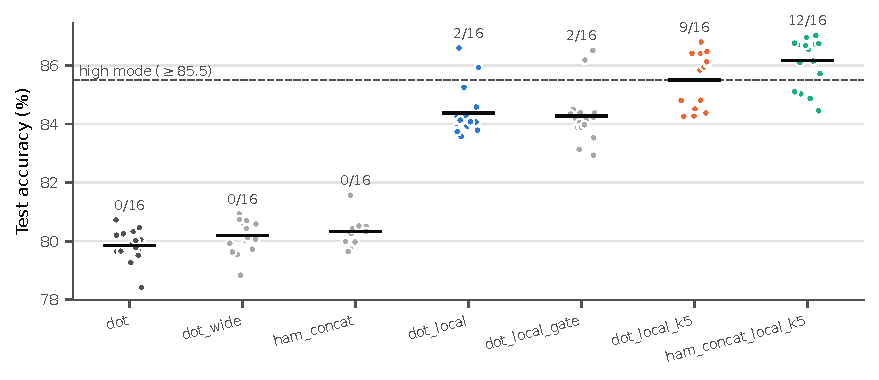
\includegraphics[width=\textwidth]{figuras/semillas.pdf}
  \caption{Test accuracy of each of the 16 seeds. Horizontal bars are the mean, and the numbers are the seeds in the high mode ($\geq 85.5$~\%, dashed line).}
  \label{fig:semillas}
\end{figure*}

\subsubsection{Generalization to PlantVillage}
\label{sec:res-pv}
On PlantVillage (Table~\ref{tab:plantvillage}), where \var{dot} already reaches 97.70~\%, the local term keeps its sign: $+0.46$ with $3\times3$ and $+0.63$ [$+0.38$, $+0.87$] with $5\times5$, 5 of 5 seeds in both cases (Holm $p=0.054$ and $0.019$, over eleven comparisons). On this dataset the additive branches also improve on \var{dot} ($+0.42$ to $+0.64$), but the pairwise branches cost 3.7 to 4.5 times the epoch time of \var{dot}, while the local term costs the same as \var{dot}. \var{dot\_local\_k5} also has the best calibration (ECE of 0.23 versus 0.39~\%) and the highest robustness to noise and blur. Its weak point is occlusion: with 25~\% of the patches erased it obtains 38.7~\%, against 44.9~\% for \var{dot} and 47 to 51~\% for the additive variants.

PlantVillage is also the only dataset on which a second similarity function contributes, and it does so on top of the local term. With the $5\times5$ convolution, the free pairwise additive reaches 98.71~\% ($+1.00$ [$+0.68$, $+1.32$] over \var{dot}) and \var{ham\_sum} 98.74~\% ($+1.04$), close to the sum of the separate effects. Over \var{dot\_local\_k5} they gain $+0.38$ [$+0.13$, $+0.62$] and $+0.42$ [$+0.17$, $+0.66$], in all 5 seeds. The contribution comes from the additive branch and not from the fusion: \var{ham\_sum} remains collapsed onto that branch and performs the same as the additive branch alone ($+0.04$ [$-0.17$, $+0.25$]). The combination costs about four times the epoch time of \var{dot\_local\_k5} and inherits both weaknesses: the occlusion weakness of the local term (38.3~\%) and the noise weakness of the additive branch (34 to 35~\%).

The capacity controls repeat on PlantVillage what was observed on CIFAR-10. Widening the MLP does not help: \var{dot\_wide} gains $+0.06$ over \var{dot} and \var{dot\_wide\_local\_k5} gains $+0.09$ over \var{dot\_local\_k5}. The neighborhood does separate from capacity ($+0.56$ [$+0.12$, $+1.00$] over \var{dot\_wide}, 5 of 5 seeds). The \emph{pooling} branch beats its equal-capacity control in all 5 seeds, without neighborhood ($+0.24$ [$+0.01$, $+0.48$], $p=0.046$) and with it: the triad reaches 98.64~\% and beats \var{dot\_wide\_local\_k5} by $+0.23$ [$-0.05$, $+0.51$] ($p=0.089$). With 5 seeds none of these differences survives correction (Table~\ref{tab:evidencia}), and on this dataset the triad is not better calibrated than its control (ECE $-0.02$). The triad ties with the free additive plus neighborhood ($-0.06$, $p=0.49$), at a third of its epoch time (9.8 versus 29.0~s) and with a lower ECE (0.22 versus 0.29~\%).

% Translated by scripts/tables_en.py from the Spanish table generated by scripts/ieee_tables.py a partir de los runs; no editar a mano.

\begin{table*}[!t]
\centering
\footnotesize
\caption{PlantVillage (38 classes, $64\times64$, 50 epochs, batch 128, seeds 0--4). $\Delta$ paired against \texttt{dot}, Holm over 11 comparisons. ECE in \%. Robustness: accuracy with Gaussian noise $\sigma=0.1$, blur $\sigma=1$~px and occlusion of 25~\% of the patches.}
\label{tab:plantvillage}
\begin{adjustbox}{max width=\linewidth}
\begin{tabular}{lccccrrrrr}
\toprule
Variant & Accuracy (\%) & $\Delta$ [95~\% CI] & $\Delta>0$ & $p$ Holm & s/epoch & ECE & Noise & Blur & Occlusion \\
\midrule
\texttt{dot} & 97.70 $\pm$ 0.25 & --- & --- & --- & 7.7 & 0.39 & 42.2 & 86.8 & 44.9 \\
\texttt{dot\_wide} & 97.77 $\pm$ 0.24 & $+0.06$ [$-0.51$, $+0.64$] & 2/5 & 0.772 & 7.8 & 0.41 & 39.8 & 87.9 & 52.1 \\
\texttt{additive} & 98.12 $\pm$ 0.07 & $+0.42$ [$+0.06$, $+0.78$] & 5/5 & 0.095 & 5.1 & 0.36 & 31.2 & 87.0 & 50.7 \\
\texttt{additive\_free} & 98.22 $\pm$ 0.09 & $+0.52$ [$+0.20$, $+0.84$] & 5/5 & 0.054 & 28.8 & 0.38 & 28.6 & 88.6 & 47.0 \\
\texttt{ham\_concat} & 98.01 $\pm$ 0.14 & $+0.31$ [$-0.11$, $+0.73$] & 5/5 & 0.220 & 9.6 & 0.29 & 40.8 & 87.8 & 49.8 \\
\texttt{ham\_sum} & 98.35 $\pm$ 0.14 & $+0.64$ [$+0.29$, $+1.00$] & 5/5 & 0.043 & 34.8 & 0.31 & 28.2 & 89.2 & 51.5 \\
\texttt{dot\_local} & 98.17 $\pm$ 0.27 & $+0.46$ [$+0.16$, $+0.76$] & 5/5 & 0.054 & 7.8 & 0.30 & 37.9 & 89.9 & 39.7 \\
\texttt{dot\_local\_k5} & 98.33 $\pm$ 0.21 & $+0.63$ [$+0.38$, $+0.87$] & 5/5 & 0.019 & 7.8 & 0.23 & 48.6 & 92.8 & 38.7 \\
\texttt{dot\_wide\_local\_k5} & 98.42 $\pm$ 0.23 & $+0.72$ [$+0.41$, $+1.02$] & 5/5 & 0.022 & 8.0 & 0.24 & 44.4 & 93.4 & 33.6 \\
\texttt{ham\_concat\_local\_k5} & 98.64 $\pm$ 0.13 & $+0.94$ [$+0.50$, $+1.38$] & 5/5 & 0.028 & 9.8 & 0.22 & 44.9 & 94.1 & 35.4 \\
\texttt{additive\_free\_local\_k5} & 98.71 $\pm$ 0.09 & $+1.00$ [$+0.68$, $+1.32$] & 5/5 & 0.011 & 29.0 & 0.29 & 33.7 & 93.7 & 38.3 \\
\texttt{ham\_sum\_local\_k5} & 98.74 $\pm$ 0.11 & $+1.04$ [$+0.68$, $+1.41$] & 5/5 & 0.014 & 32.3 & 0.30 & 35.3 & 93.2 & 38.3 \\
\bottomrule
\end{tabular}
\end{adjustbox}
\end{table*}


\subsubsection{Training Efficiency}
\label{sec:res-eficiencia}
The local term also speeds up learning (Fig.~\ref{fig:curvas}, Table~\ref{tab:eficiencia}). \var{dot} reaches 79~\% validation accuracy at epoch 234 on average (15 of 16 seeds reach it); \var{dot\_local} does so at epoch 75 and \var{dot\_local\_k5} at epoch 59, which amounts to 88~s of GPU time against 323~s, 3.7 times less. Trained for only 100 epochs, \var{dot\_local} reaches 80.01 $\pm$ 0.34~\%, the same as \var{dot} with 400 epochs ($-0.03$ [$-0.50$, $+0.44$], paired by seed). \var{ham\_concat\_local\_k5} needs the fewest epochs (55), but, because of its cost per epoch, not the least GPU time: 136~s, 2.4 times less than \var{dot}, against 3.7 times for \var{dot\_local\_k5}.

\begin{figure}[tbp]
  \centering
  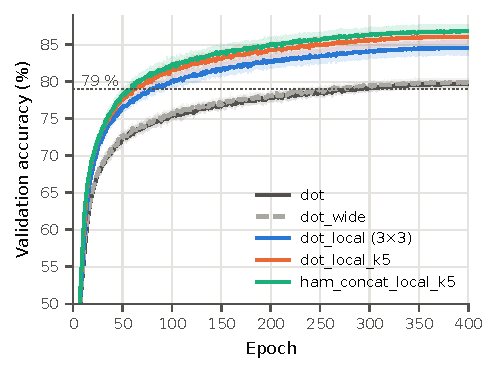
\includegraphics[width=\anchocolumna]{figuras/curvas.pdf}
  \caption{Validation accuracy per epoch on CIFAR-10 (mean $\pm$ standard deviation of 16 seeds). The dotted line marks 79~\%, close to the final value of \var{dot}. The curves of \var{dot} and \var{dot\_wide} overlap.}
  \label{fig:curvas}
\end{figure}

% Translated by scripts/tables_en.py from the Spanish table generated by scripts/ieee_tables.py a partir de los runs; no editar a mano.

\begin{table*}[!t]
\centering
\small
\caption{Training efficiency on CIFAR-10. Epoch and GPU time to reach 79~\% validation accuracy (16 seeds; in parentheses, how many reach it when not all do). Test accuracy when training for 100 epochs (3 warmup epochs; seeds 0--4) and 400 epochs (16 seeds).}
\label{tab:eficiencia}
\begin{adjustbox}{max width=\linewidth}
\begin{tabular}{lcccc}
\toprule
Variant & Epoch $\geq$79 & Time (s) & 100 epochs & 400 epochs \\
\midrule
\texttt{dot} & 234 (15/16) & 323 & 75.85 $\pm$ 0.27 & 79.85 $\pm$ 0.54 \\
\texttt{dot\_wide} & 213 (15/16) & 301 & 76.03 $\pm$ 0.38 & 80.19 $\pm$ 0.56 \\
\texttt{ham\_concat} & 204 & 474 & --- & 80.34 $\pm$ 0.43 \\
\texttt{dot\_local} & 75 & 111 & 80.01 $\pm$ 0.34 & 84.38 $\pm$ 0.84 \\
\texttt{dot\_local\_k5} & 59 & 88 & --- & 85.49 $\pm$ 0.90 \\
\texttt{dot\_wide\_local\_k5} & 57 & 87 & --- & 85.67 $\pm$ 1.02 \\
\texttt{ham\_concat\_local\_k5} & 55 & 136 & --- & 86.16 $\pm$ 0.86 \\
\texttt{dot\_local\_gate} & 70 & 108 & 80.13 $\pm$ 0.28 & 84.27 $\pm$ 0.92 \\
\bottomrule
\end{tabular}
\end{adjustbox}
\end{table*}


\subsubsection{Computational Cost and Inference}
\label{sec:res-costos}
Table~\ref{tab:costos} separates the cost of the variants into hardware-independent quantities and inference measurements. The $5\times5$ local term adds 3.4~\% of MACs (9.27 versus 8.96 million per image) and 4.2~\% of parameters, and it does not change the peak memory of a training step (624~MB) or that of activations (256~KB); its epoch time (1.08 times) is consistent with that arithmetic. The triad, on the other hand, has the same MACs as its capacity control ($+10.3$ versus $+10.4$~\%) and the same memory, but 1.79 times the epoch time against 1.10: the difference comes from the implementation of the \emph{pooling} branch, computed head by head, not from its arithmetic. The opposite happens with the score fusions with pairwise additive attention: \var{ham\_sum} has the MACs of \var{dot}, because the counter does not see the element-wise $\tanh$ over $N\times N\times d$ tensors, but it needs 2.3 times the training memory and 2.5 times the activation memory. Parameter count and MACs are therefore not enough to judge the cost of an attention mechanism.

At inference, with batch 1 and one CPU thread, the models take 0.55 to 2.5~ms per image and weigh about 0.5~MB in fp32. At this size, latency depends more on the number of operations launched than on the arithmetic: the local term adds 27~\% of latency (from 0.67 to 0.85~ms) for 3.4~\% of MACs, and the ResNet, with 2.2 times the MACs of \var{dot}, is the fastest (0.55~ms; 0.28~ms with 16 threads), because each convolution runs as a single optimized kernel. As the model grows, the relative cost of the local term falls: at 3.6 million parameters it adds 1.0~\% of MACs and 8~\% of CPU latency. These measurements come from a desktop CPU with PyTorch in eager mode; they do not indicate the latency or memory on a microcontroller or an NPU, where quantization, the compiler and the available operators may change the ranking.

% Translated by scripts/tables_en.py from the Spanish table generated by scripts/ieee_tables.py a partir de los runs; no editar a mano.

\begin{table*}[!t]
\centering
\small
\caption{Cost of each variant on CIFAR-10. Hardware-independent: MACs per image at inference and training FLOPs per epoch (\emph{forward} and \emph{backward} over 45{,}000 images), counting matrix products and convolutions, not element-wise operations. Peak memory of a training step (batch 256, fp32, AdamW) and epoch time relative to \texttt{dot} (seeds 0--4), on an RTX 5080. Inference with batch 1: median CPU latency with one thread (AMD Ryzen 7 9700X, 300 repetitions), peak activation memory and model size on disk (fp32).}
\label{tab:costos}
\begin{adjustbox}{max width=\linewidth}
\begin{tabular}{lrrrrrrrrr}
\toprule
Variant & Params. & MMACs & $\Delta$ MACs & TFLOPs/epoch & Mem. (MB) & s/epoch & CPU (ms) & Activ. (KB) & Disk (KB) \\
\midrule
\texttt{dot} & 119\,290 & 8.96 & --- & 2.41 & 624 & 1.00$\times$ & 0.67 & 256 & 490 \\
\texttt{dot\_wide} & 128\,990 & 9.58 & +7.0~\% & 2.57 & 658 & 1.02$\times$ & 0.69 & 282 & 528 \\
\texttt{ham\_concat} & 128\,906 & 9.57 & +6.8~\% & 2.57 & 663 & 1.68$\times$ & 1.05 & 256 & 564 \\
\texttt{ham\_sum} & 119\,290 & 8.96 & +0.0~\% & 2.41 & 1416 & 1.95$\times$ & 2.53 & 644 & 495 \\
\texttt{dot\_local} & 121\,210 & 9.07 & +1.2~\% & 2.44 & 624 & 1.07$\times$ & 0.84 & 256 & 501 \\
\texttt{dot\_local\_k5} & 124\,282 & 9.27 & +3.4~\% & 2.49 & 624 & 1.08$\times$ & 0.85 & 256 & 513 \\
\texttt{dot\_wide\_local\_k5} & 133\,982 & 9.89 & +10.4~\% & 2.66 & 656 & 1.10$\times$ & 0.87 & 282 & 550 \\
\texttt{ham\_concat\_local\_k5} & 133\,898 & 9.88 & +10.3~\% & 2.65 & 664 & 1.79$\times$ & 1.24 & 256 & 587 \\
\midrule
\texttt{localvit} & 126\,970 & 9.40 & +4.9~\% & 2.53 & 876 & 1.39$\times$ & 0.97 & 302 & 523 \\
\texttt{spt\_lsa} & 129\,002 & 9.55 & +6.6~\% & 2.58 & 723 & 1.24$\times$ & 0.75 & 256 & 533 \\
\texttt{convit} & 124\,398 & 9.28 & +3.6~\% & 2.49 & 654 & 1.54$\times$ & 1.34 & 269 & 519 \\
\texttt{conv\_stem} & 130\,450 & 9.79 & +9.3~\% & 2.63 & 644 & 1.06$\times$ & 0.70 & 256 & 538 \\
\texttt{resnet} & 121\,390 & 19.40 & +116.5~\% & 5.19 & 296 & 0.75$\times$ & 0.55 & 320 & 495 \\
\bottomrule
\end{tabular}
\end{adjustbox}
\end{table*}


\subsection{Scope of the Results}
\label{sec:res-alcance}
The results above come from a single model, a main dataset and one augmentation protocol. This subsection tests them in four directions, with seeds 0 to 4: other augmentation protocols, other locality mechanisms with the same parameter budget, other datasets, and other scales of data and model.

\subsubsection{Comparison with Published Locality Mechanisms}
\label{sec:res-baselines}
Table~\ref{tab:baselines} compares the local term with four published ways of giving locality to a small ViT and with a ResNet of the same size, all implemented with between 119,000 and 134,000 parameters and trained with the same protocol:
\begin{itemize}
  \item LocalViT, a depthwise convolution in the MLP;
  \item SPT+LSA, shifted-patch tokenization and attention with a learned temperature;
  \item ConViT, attention with convolutional initialization and a gate;
  \item a convolutional stem instead of the patch projection;
  \item a three-stage ResNet.
\end{itemize}
The term in the attention output and the LocalViT term in the MLP perform equally (LocalViT $+0.51$ [$-1.05$, $+2.07$], 3 of 5 seeds), but ours costs 1.08 times the epoch time of \var{dot} and LocalViT 1.39. Locality only at the input contributes little: the convolutional stem improves on \var{dot} by 2.0 points, with the worst ECE in the table (9.17~\%), and SPT+LSA by 1.0. ConViT, whose locality is an initialization that attention can abandon, lies in between ($+4.1$ over \var{dot}, at 1.54 times its cost). What separates the mechanisms is whether the neighborhood is present in every block throughout training, more than the place in the block where it is introduced. The ResNet, with 121,390 parameters and a convolutional bias in every layer, beats all the ViTs: 87.14~\%, $+1.77$ [$+0.31$, $+3.23$] over \var{dot\_local\_k5} in all 5 seeds, with the lowest epoch time (0.75 times that of \var{dot}). The local term closes 75~\% of the gap between \var{dot} and the ResNet, and the triad 94~\%.

% Translated by scripts/tables_en.py from the Spanish table generated by scripts/ieee_tables.py a partir de los runs; no editar a mano.

\begin{table*}[!t]
\centering
\small
\caption{Comparison with published locality mechanisms at the same parameter budget (119k--134k) and with the same training protocol (CIFAR-10, 400 epochs, seeds 0--4). $\Delta$ paired against \texttt{dot\_local\_k5}; Holm over the comparisons in the table. Cost: epoch time relative to \texttt{dot}. ECE in \%.}
\label{tab:baselines}
\begin{adjustbox}{max width=\linewidth}
\begin{tabular}{llrcccccc}
\toprule
Variant & Mechanism & Params. & Accuracy (\%) & $\Delta$ [95~\% CI] & $\Delta>0$ & $p$ Holm & Cost & ECE \\
\midrule
\texttt{dot} & Base ViT & 119\,290 & 80.04 $\pm$ 0.31 & $-5.32$ [$-6.81$, $-3.84$] & 0/5 & 0.004 & 1.00$\times$ & 6.55 \\
\texttt{dot\_wide} & Base ViT, MLP 217 & 128\,990 & 79.73 $\pm$ 0.63 & $-5.64$ [$-7.30$, $-3.98$] & 0/5 & 0.004 & 1.02$\times$ & 6.95 \\
\texttt{dot\_local\_k5} & This work & 124\,282 & 85.36 $\pm$ 1.16 & --- & --- & --- & 1.08$\times$ & 5.28 \\
\texttt{ham\_concat\_local\_k5} & This work (triad) & 133\,898 & 86.68 $\pm$ 0.55 & $+1.32$ [$-0.04$, $+2.68$] & 4/5 & 0.162 & 1.79$\times$ & 4.93 \\
\midrule
\texttt{localvit} & LocalViT \cite{li2021localvit} & 126\,970 & 85.88 $\pm$ 0.38 & $+0.51$ [$-1.05$, $+2.07$] & 3/5 & 0.413 & 1.39$\times$ & 6.04 \\
\texttt{spt\_lsa} & SPT + LSA \cite{lee2021vision} & 129\,002 & 81.08 $\pm$ 0.43 & $-4.29$ [$-5.82$, $-2.75$] & 0/5 & 0.007 & 1.24$\times$ & 5.97 \\
\texttt{convit} & ConViT \cite{dascoli2021convit} & 124\,398 & 84.11 $\pm$ 1.05 & $-1.26$ [$-2.81$, $+0.29$] & 1/5 & 0.174 & 1.54$\times$ & 5.07 \\
\texttt{conv\_stem} & Conv.\ stem \cite{xiao2021early} & 130\,450 & 82.08 $\pm$ 0.87 & $-3.29$ [$-3.94$, $-2.64$] & 0/5 & 0.001 & 1.06$\times$ & 9.17 \\
\texttt{resnet} & ResNet \cite{he2016deep} & 121\,390 & 87.14 $\pm$ 0.19 & $+1.77$ [$+0.31$, $+3.23$] & 5/5 & 0.112 & 0.75$\times$ & 5.42 \\
\bottomrule
\end{tabular}
\end{adjustbox}
\end{table*}


\subsubsection{Data Augmentation: CutMix Does Not Replace the Neighborhood}
\label{sec:res-aumento}
In a 2.4-million-parameter ViT, CutMix suffices for local attention heads to appear \cite{santiago2026inducing}. If the same happened in this model, the local term could be redundant with suitable data augmentation. Table~\ref{tab:aumento} repeats the five key variants with CutMix ($\alpha=1$, probability 0.6, the same protocol) and with a strong augmentation (RandAugment \cite{cubuk2020randaugment}, CutMix \cite{yun2019cutmix} or Mixup \cite{zhang2018mixup} on each batch, and label smoothing \cite{szegedy2016rethinking} of 0.1).
\begin{itemize}
  \item \textbf{CutMix does not change the accuracy of \var{dot}} (80.08 versus 80.04~\%) \textbf{and does not induce local heads.} Across the four layers and the five seeds, the most local head of \var{dot} attends at a mean distance of 11.0 to 11.6~pixels under any of the three protocols. With uniform attention over the $8\times8$ grid that distance is 16.5~pixels, and CutMix reduces it by less than 0.5.
  \item \textbf{With CutMix, the neighborhood still contributes} $+4.58$ [$+3.30$, $+5.87$] over \var{dot\_wide}, in all 5 seeds.
  \item \textbf{CutMix does improve calibration substantially.} The ECE of \var{dot} drops from 6.55 to 2.48~\% and that of \var{dot\_local\_k5} from 5.28 to 1.59~\%. With CutMix, the triad is better calibrated than its capacity control (ECE $-0.50$, $p=0.007$) and beats it in accuracy by $+1.47$ [$+0.01$, $+2.92$].
  \item \textbf{Strong augmentation is too much regularization for 119,000 parameters.} All variants lose 1.6 to 3 points. The models become underconfident: \var{dot} has a mean confidence of 64~\% with 77~\% accuracy, and ECE rises to 12.7--14.9~\%. Even so, the neighborhood contributes $+6.42$ points.
\end{itemize}
The difference from the 2.4-million-parameter result is probably one of scale, but this was not tested. With 119,000 parameters and 45,000 images, the neighborhood bias has to be in the architecture.

% Translated by scripts/tables_en.py from the Spanish table generated by scripts/ieee_tables.py a partir de los runs; no editar a mano.

\begin{table*}[!t]
\centering
\small
\caption{Effect of the augmentation protocol on CIFAR-10 (seeds 0--4, 400 epochs). CutMix: $\alpha=1$ with probability 0.6, as in \cite{santiago2026inducing}. Strong augmentation: RandAugment, CutMix or Mixup on each batch, and label smoothing 0.1. Neighborhood: \texttt{dot\_local\_k5} $-$ \texttt{dot\_wide}; triad: \texttt{ham\_concat\_local\_k5} $-$ \texttt{dot\_wide\_local\_k5}. Distance: mean attention distance (px) of the most local head in layer 1; uniform attention would give 16.5~px.}
\label{tab:aumento}
\begin{adjustbox}{max width=\linewidth}
\begin{tabular}{lcccccccc}
\toprule
Protocol & \texttt{dot} & \texttt{dot\_local\_k5} & $\Delta$ neighborhood [95~\% CI] & $\Delta>0$ & Triad & $\Delta$ triad [95~\% CI] & $\Delta>0$ & Distance (\texttt{dot} / local) \\
\midrule
Standard & 80.04 $\pm$ 0.31 & 85.36 $\pm$ 1.16 & $+5.64$ [$+3.98$, $+7.30$] & 5/5 & 86.68 $\pm$ 0.55 & $+1.03$ [$-1.02$, $+3.09$] & 4/5 & 14.2 / 14.3 \\
CutMix & 80.08 $\pm$ 0.26 & 85.21 $\pm$ 1.09 & $+4.58$ [$+3.30$, $+5.87$] & 5/5 & 86.39 $\pm$ 1.00 & $+1.47$ [$+0.01$, $+2.92$] & 4/5 & 13.7 / 14.2 \\
Strong aug. & 76.99 $\pm$ 0.35 & 83.73 $\pm$ 1.18 & $+6.42$ [$+4.91$, $+7.92$] & 5/5 & 83.93 $\pm$ 0.78 & $+0.29$ [$-1.30$, $+1.89$] & 3/5 & 13.9 / 14.6 \\
\bottomrule
\end{tabular}
\end{adjustbox}
\end{table*}


\subsubsection{Other Datasets}
\label{sec:res-datos}
Table~\ref{tab:datos} repeats the five variants on CIFAR-100 (400 epochs) and on SVHN \cite{netzer2011reading} (100 epochs, without horizontal flip, because it mirrors the digits), and gathers CIFAR-10 and PlantVillage with the same seeds. The neighborhood separates from the capacity control on all four datasets: $+5.38$ [$+4.62$, $+6.14$] on CIFAR-100, $+2.77$ [$+2.00$, $+3.53$] on SVHN and $+0.56$ on PlantVillage, in every seed. The triad over its control gives $+0.32$ on CIFAR-100, with a lower ECE ($-0.71$, $p=0.086$), and ties on SVHN ($-0.00$ [$-0.25$, $+0.25$]), the dataset on which all the variants with neighborhood end within 0.02 points of each other.

% Translated by scripts/tables_en.py from the Spanish table generated by scripts/ieee_tables.py a partir de los runs; no editar a mano.

\begin{table*}[!t]
\centering
\small
\caption{Test accuracy (\%) on four datasets, seeds 0--4. CIFAR-100: 400 epochs; SVHN: 100 epochs, no flip; PlantVillage: 50 epochs, batch 128. Neighborhood: \texttt{dot\_local\_k5} $-$ \texttt{dot\_wide}; triad: \texttt{ham\_concat\_local\_k5} $-$ \texttt{dot\_wide\_local\_k5}.}
\label{tab:datos}
\begin{adjustbox}{max width=\linewidth}
\begin{tabular}{lccccccccc}
\toprule
Dataset & \texttt{dot} & \texttt{dot\_wide} & \texttt{dot\_local\_k5} & \texttt{dot\_wide\_local\_k5} & Triad & $\Delta$ neighborhood & $\Delta>0$ & $\Delta$ triad & $\Delta>0$ \\
\midrule
CIFAR-10 & 80.04 $\pm$ 0.31 & 79.73 $\pm$ 0.63 & 85.36 $\pm$ 1.16 & 85.65 $\pm$ 1.23 & 86.68 $\pm$ 0.55 & $+5.64$ [$+3.98$, $+7.30$] & 5/5 & $+1.03$ [$-1.02$, $+3.09$] & 4/5 \\
CIFAR-100 & 51.34 $\pm$ 0.43 & 51.96 $\pm$ 0.58 & 57.34 $\pm$ 0.92 & 57.63 $\pm$ 0.68 & 57.95 $\pm$ 1.01 & $+5.38$ [$+4.62$, $+6.14$] & 5/5 & $+0.32$ [$-1.09$, $+1.73$] & 3/5 \\
SVHN & 93.49 $\pm$ 0.49 & 93.25 $\pm$ 0.63 & 96.02 $\pm$ 0.06 & 96.04 $\pm$ 0.14 & 96.04 $\pm$ 0.20 & $+2.77$ [$+2.00$, $+3.53$] & 5/5 & $-0.00$ [$-0.25$, $+0.25$] & 3/5 \\
PlantVillage & 97.70 $\pm$ 0.25 & 97.77 $\pm$ 0.24 & 98.33 $\pm$ 0.21 & 98.42 $\pm$ 0.23 & 98.64 $\pm$ 0.13 & $+0.56$ [$+0.12$, $+1.00$] & 5/5 & $+0.23$ [$-0.05$, $+0.51$] & 5/5 \\
\bottomrule
\end{tabular}
\end{adjustbox}
\end{table*}


\subsubsection{Data Fraction and Model Size}
\label{sec:res-escala}
Table~\ref{tab:escala} varies the amount of CIFAR-10 training data (10, 25, 50 and 100~\% of the 45,000 images, with a fixed subset for all seeds) and the model size ($D\in\{48,96,192\}$ and $L\in\{4,8\}$, from 119,000 to 3.6 million parameters).

Contrary to the intuition that an inductive bias matters more when data are scarce, the gain of the neighborhood grows with the data: $+2.77$ with 10~\%, $+3.90$ with 25~\%, $+5.17$ with 50~\% and $+5.32$ with 100~\%, in every seed. It also grows in relative terms: the error reduction goes from 7 to 27~\%. With 4,500 images both models overfit (training accuracy of 83 to 90~\% and validation accuracy of 58 to 62~\%), and the amount of data is more limiting than the architecture.

The gain does not shrink with model size. It ranges from $+5.10$ to $+7.21$ points across the six sizes, in every seed, and its cost is 1.05 to 1.08 times the epoch time of \var{dot} of the same size and 1.0 to 3.5~\% of MACs. \var{dot\_local\_k5} with 124,282 parameters (85.36~\%) beats \var{dot} with 3.6 million (83.37~\%). In this range, enlarging the model does not replace the neighborhood bias.

% Translated by scripts/tables_en.py from the Spanish table generated by scripts/ieee_tables.py a partir de los runs; no editar a mano.

\begin{table*}[!t]
\centering
\small
\caption{Gain of the $5\times5$ local term by fraction of the CIFAR-10 training set (top, seeds 0--4, 400 epochs) and by model size (bottom, 4 heads and an MLP of $4D$, seeds 0--2). Parameters of \texttt{dot}. Triad: \texttt{ham\_concat\_local\_k5} $-$ \texttt{dot\_wide\_local\_k5}.}
\label{tab:escala}
\begin{adjustbox}{max width=\linewidth}
\begin{tabular}{lrcccccc}
\toprule
Configuration & Params. & \texttt{dot} & \texttt{dot\_local\_k5} & $\Delta$ local [95~\% CI] & $\Delta>0$ & $\Delta$ triad & $\Delta>0$ \\
\midrule
10~\% of the data & 119\,290 & 59.48 $\pm$ 0.54 & 62.25 $\pm$ 0.56 & $+2.77$ [$+1.84$, $+3.71$] & 5/5 & $+1.29$ [$-1.19$, $+3.78$] & 4/5 \\
25~\% of the data & 119\,290 & 69.53 $\pm$ 0.47 & 73.44 $\pm$ 0.49 & $+3.90$ [$+3.15$, $+4.66$] & 5/5 & $+1.37$ [$-0.61$, $+3.34$] & 5/5 \\
50~\% of the data & 119\,290 & 74.80 $\pm$ 0.46 & 79.97 $\pm$ 1.15 & $+5.17$ [$+3.89$, $+6.44$] & 5/5 & $+1.39$ [$-0.29$, $+3.08$] & 4/5 \\
100~\% of the data & 119\,290 & 80.04 $\pm$ 0.31 & 85.36 $\pm$ 1.16 & $+5.32$ [$+3.84$, $+6.81$] & 5/5 & $+1.03$ [$-1.02$, $+3.09$] & 4/5 \\
\midrule
$D=48$, $L=4$ & 119\,290 & 80.10 $\pm$ 0.33 & 85.20 $\pm$ 1.39 & $+5.10$ [$+1.99$, $+8.21$] & 3/3 & --- & --- \\
$D=96$, $L=4$ & 459\,754 & 81.75 $\pm$ 0.53 & 88.10 $\pm$ 0.08 & $+6.35$ [$+5.20$, $+7.50$] & 3/3 & --- & --- \\
$D=192$, $L=4$ & 1\,804\,234 & 83.23 $\pm$ 0.60 & 89.12 $\pm$ 0.37 & $+5.89$ [$+4.03$, $+7.76$] & 3/3 & --- & --- \\
$D=48$, $L=8$ & 232\,378 & 80.53 $\pm$ 0.13 & 87.74 $\pm$ 0.34 & $+7.21$ [$+6.56$, $+7.85$] & 3/3 & --- & --- \\
$D=96$, $L=8$ & 907\,114 & 80.98 $\pm$ 0.42 & 88.17 $\pm$ 1.28 & $+7.19$ [$+3.85$, $+10.54$] & 3/3 & --- & --- \\
$D=192$, $L=8$ & 3\,583\,690 & 83.37 $\pm$ 0.98 & 89.88 $\pm$ 0.28 & $+6.51$ [$+3.82$, $+9.19$] & 3/3 & --- & --- \\
\bottomrule
\end{tabular}
\end{adjustbox}
\end{table*}


\subsubsection{The Triad Against Its Control in All Conditions}
\label{sec:res-triada-condiciones}
In the nine conditions of this subsection (the three augmentation protocols, the three data fractions and the four datasets, with standard CIFAR-10 in common), the triad beats its equal-capacity control on average in eight, and ties on SVHN. Outside standard CIFAR-10, which is part of the primary contrast, it wins in 31 of the 40 seed pairs, with a mean difference of $+0.79$ points across the eight conditions. The conditions share seeds and, for the most part, images, so this aggregate is exploratory. What it shows is that the sign of the primary contrast ($+0.61$ with 48 seeds) recurs outside it. None of the conditions, with 5 seeds, separates on its own after correction.

\subsection{Analysis of the Attention Mechanism}
\label{sec:res-atencion}

\subsubsection{Representative Attention Maps}
\label{sec:res-mapas}
Two trainings of the same model can produce CLS \emph{attention-rollout} maps that differ as much as those of two variants (Supplementary Fig.~\ref{fig:mapas}), so the maps are compared quantitatively, against the between-seed variation of each variant (Supplementary Section~\ref{sec:sup-mapas}). The models with a local term have maps that are more reproducible across seeds than those of \var{dot}, and their distance to \var{dot} exceeds the between-seed variation of \var{dot} by a factor of 1.2 to 1.6: the local term produces maps that differ from those of \var{dot} and are consistent across seeds. The fusions of the first family, by contrast, differ from \var{dot} only as much as their own seeds differ from each other.

\subsubsection{Behavior Across Layers}
\label{sec:res-capas}
Fig.~\ref{fig:mecanismo} summarizes the attention per layer. In \var{dot}, the second and third layers are the most selective (normalized entropy of 0.83 and 0.86) and those with the highest diversity between heads (JS of 0.36 and 0.29). With the local term, the attention of those layers becomes more uniform (0.92--0.93 in layer 2) and the heads become more alike (JS of 0.18--0.22 in layer 2). The mean attention distance is 14 to 17~pixels in all variants, on 32-pixel images: attention is global with and without the local term. We read this as a division of labor: when the convolution handles the mixing between neighbors, the heads stop specializing in different local patterns and attention is left to handle global relations.

The local term contributes between 45 and 47~\% of the output norm in layers 1 to 3 with $3\times3$, between 47 and 55~\% with $5\times5$, and between 54 and 61~\% in \var{ham\_concat\_local\_k5}; in layer 4 it contributes zero (Section~\ref{sec:terminos}). In the \var{dot\_local\_k1} control the term is also used (23 to 38~\%), but the attention is the same as in \var{dot}: without mixing neighbors, the additional value path does not change what attention does. In \var{ham\_concat\_local\_k5} the \emph{pooling} branch provides between 37 and 49~\% of the fusion output, almost the same as in \var{ham\_concat} (40 to 47~\%).

\begin{figure*}[!t]
  \centering
  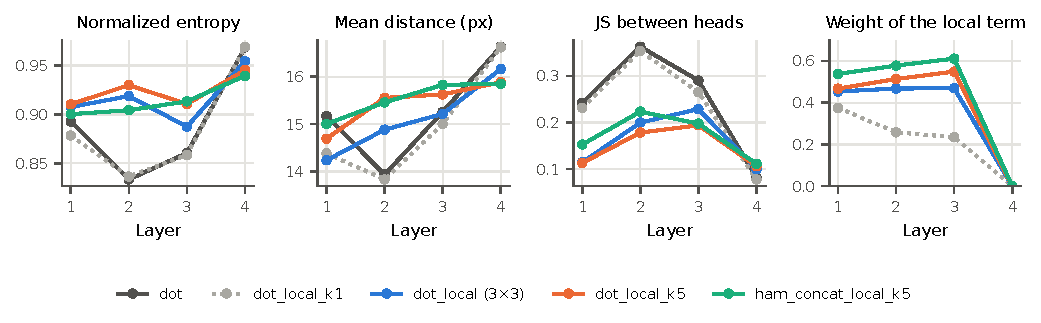
\includegraphics[width=\textwidth]{figuras/mecanismo.pdf}
  \caption{Attention per layer on CIFAR-10 (mean of 16 seeds; 5 for \var{dot\_local\_k1}). From left to right: normalized entropy of the attention rows, mean attention distance, JS divergence between heads and fraction of the output norm contributed by the local term.}
  \label{fig:mecanismo}
\end{figure*}

\subsubsection{Comparison with the Fusion Mechanisms}
\label{sec:res-colapso}
Table~\ref{tab:colapso} explains why the fusions of the first family do not improve on \var{dot}. In score mixing, one of the two branches dominates and the other becomes irrelevant; which one wins depends on the relative scale of the scores:
\begin{itemize}
  \item with $\lambda=0.85$, the applied attention is almost that of \var{dot} (JS of 0.016--0.035) and far from the additive one (0.27--0.39);
  \item with the sum, the free additive, whose scores reach $\pm d$, dominates (JS of 0.005--0.056) and the \var{dot} branch becomes almost uniform (entropy of 0.96--1.00);
  \item when the additive branch is scaled by $1/\sqrt{d}$, it flattens (entropy of 0.94--0.97) and \var{dot} wins (JS of 0.001--0.004).
\end{itemize}
This is the expected consequence of score mixing being a product of distributions (Section~\ref{sec:fusiones}): the sharper branch decides. Standardizing the scores (\var{ham\_zscore}) and mixing outputs instead of scores avoid the collapse: the applied attention differs from both branches and the \var{dot} branch contributes between 60 and 77~\% of the output. But they do not improve accuracy either (Table~\ref{tab:fusiones}). Moreover, when $\lambda$ is learned, its final value depends on the initialization: the same output-mixing model ends with $\lambda_{\text{dot}}$ of 0.65--0.76 if it starts at 0.85, and of 0.23--0.40 if it starts at 0.5, with a 0.79-point difference in accuracy (5 of 5 seeds, $p=0.007$). The problem with these fusions is not only collapse: two similarity functions computed on the same queries and keys do not provide complementary information.

% Translated by scripts/tables_en.py from the Spanish table generated by scripts/ieee_tables.py a partir de los runs; no editar a mano.

\begin{table*}[!t]
\centering
\footnotesize
\caption{Use of the two branches in the CIFAR-10 fusions (mean over seeds 0--4; range over the 4 layers). JS: Jensen--Shannon divergence (base 2) between the attention applied to $v$ and each branch. $H$: normalized entropy of each branch (1 = uniform). Contribution: fraction of the output norm contributed by \texttt{dot}, in output fusions.}
\label{tab:colapso}
\begin{adjustbox}{max width=\linewidth}
\begin{tabular}{lccccc}
\toprule
Variant & JS(fus., dot) & JS(fus., additive) & $H$ dot & $H$ additive & Contrib. dot \\
\midrule
\texttt{ham\_weighted} & 0.016--0.035 & 0.274--0.391 & 0.86--0.97 & 0.57--0.68 & --- \\
\texttt{ham\_weighted\_learn} & 0.058--0.118 & 0.219--0.292 & 0.87--0.97 & 0.59--0.70 & --- \\
\texttt{ham\_sum} & 0.115--0.254 & 0.005--0.056 & 0.96--1.00 & 0.82--0.92 & --- \\
\texttt{ham\_weighted\_scaled} & 0.001--0.004 & 0.044--0.165 & 0.81--0.96 & 0.94--0.97 & --- \\
\texttt{ham\_zscore} & 0.130--0.282 & 0.079--0.186 & 1.00 & 0.90--0.99 & --- \\
\texttt{ham\_weighted\_learn\_out} & 0.022--0.042 & 0.085--0.221 & 0.85--0.97 & 0.71--0.84 & 0.60--0.73 \\
\texttt{ham\_wout} & 0.009--0.045 & 0.086--0.215 & 0.82--0.96 & 0.75--0.84 & 0.60--0.76 \\
\texttt{ham\_gated} & 0.012--0.054 & 0.098--0.230 & 0.83--0.96 & 0.77--0.85 & 0.63--0.77 \\
\texttt{ham\_concat} & --- & --- & 0.85--0.96 & 0.78--0.85 & 0.53--0.60 \\
\bottomrule
\end{tabular}
\end{adjustbox}
\end{table*}


\subsection{Ablations of the Output Terms}
\label{sec:res-ablacion}
Ablations with seeds 0 to 4 (Supplementary Section~\ref{sec:sup-ablacion}, Table~\ref{tab:ablacion} and Fig.~\ref{fig:kernel}) locate the gain of the output terms:
\begin{itemize}
  \item \textbf{It comes from the neighborhood.} With $k=1$ (\var{dot\_local\_k1}), the term keeps the additional value path but does not mix neighboring patches, and the accuracy is that of \var{dot} ($+0.07$ [$-0.52$, $+0.67$]).
  \item \textbf{It saturates at $5\times5$.} A $7\times7$ kernel, which almost covers the $8\times8$ grid, is only $+0.20$ [$-1.19$, $+1.60$] from $5\times5$.
  \item \textbf{It is not a capacity effect.} With 16 paired seeds, \var{dot\_wide\_local\_k5} is $+0.17$ [$-0.59$, $+0.94$] from \var{dot\_local\_k5}.
  \item \textbf{The gate and the residual global context do not help}, either alone or on top of the local term; with 16 seeds, the gate on top of the local term gives $-0.11$ [$-0.50$, $+0.28$].
  \item \textbf{Other ways of combining mechanisms with the local term do not separate from it.} With 16 seeds, splitting the branches across heads gives $+0.19$ [$-0.49$, $+0.87$] over \var{dot\_local\_k5}, and removing pairwise attention altogether (only the \emph{pooling} branch with the local term, without any $N\times N$ matrix) gives $-0.47$ [$-1.24$, $+0.30$], still $+5.17$ over \var{dot}.
\end{itemize}

\subsection{Fulfillment of the Criteria}
\label{sec:res-criterios}
No variant meets all four criteria set in advance (Table~\ref{tab:criterios}). \var{dot\_local\_k5} meets the gain over the capacity control, the sign on another dataset and the cost; the per-branch contribution criterion does not apply because it has a single attention branch, and its local term contributes 47 to 55~\% of the output in layers 1 to 3. \var{ham\_concat\_local\_k5} meets three: the gain over its capacity control (with the 48 seeds, Holm $p=0.031$), the balance between branches and the same sign of that contrast on PlantVillage ($+0.23$ over \var{dot\_wide\_local\_k5}); it fails the cost criterion, at 1.78 times the epoch time of \var{dot}. \var{ham\_concat} meets the branch balance and the sign on PlantVillage ($+0.24$ over \var{dot\_wide}), but does not separate from its capacity control on CIFAR-10 and costs 1.68 times the epoch time of \var{dot}. The score fusions only meet the sign criterion, because they improve on \var{dot} on PlantVillage.

% Translated by scripts/tables_en.py from the Spanish table generated by scripts/ieee_tables.py a partir de los runs; no editar a mano.

\begin{table*}[!t]
\centering
\footnotesize
\caption{Fulfillment of the four criteria set in advance (Section~\ref{sec:analisis}). C1: paired gain on CIFAR-10 over the equal-capacity control (\texttt{dot} for score fusions, which add no parameters) with Holm $<0.05$ over the 8 comparisons and at least 10 seeds. C2: no branch contributes less than 10\,\% of the output norm; for score fusions, which have no separate outputs, the JS divergence between the applied attention and each branch is used (JS $\approx0$: the fusion is that branch); n/a: a single attention branch. C3: the C1 contrast, against the same control, has $\Delta>0$ on another dataset (PV: PlantVillage, batch 128; Food: Food-101; seeds 0--4, paired t-test $p$ in parentheses). C4: epoch time $<1.5$ times that of \texttt{dot}.}
\label{tab:criterios}
\begin{adjustbox}{max width=\linewidth}
\begin{tabular}{>{\raggedright\arraybackslash}p{3.25cm}>{\raggedright\arraybackslash}p{3.5cm}c>{\raggedright\arraybackslash}p{2.85cm}c>{\raggedright\arraybackslash}p{3.0cm}ccc}
\toprule
Variant & C1: gain &  & C2: contribution per branch &  & C3: other datasets &  & C4: cost &  \\
\midrule
\texttt{ham\_weighted} & $-0.38$, Holm 0.367 & no & fusion = \texttt{dot} (JS $\leq$0.035) & no & PV: $+0.08$ (0.534)\newline Food: not evaluated & yes & 1.89$\times$ & no \\
\texttt{ham\_sum} & $-0.55$, Holm 0.077 & no & fusion = \texttt{additive\_free} (JS $\leq$0.056) & no & PV: $+0.64$ (0.007)\newline Food: not evaluated & yes & 1.95$\times$ & no \\
\texttt{ham\_concat} & $+0.48$, Holm 0.017\newline vs.\ \texttt{dot\_wide}: $+0.15$, Holm 0.491 ($n=16$) & no & minor branch: 0.40 & yes & PV: $+0.24$ (0.046)\newline Food: control not evaluated & yes & 1.68$\times$ & no \\
\texttt{dot\_local\_k5} & $+5.64$, Holm $<0.001$\newline vs.\ \texttt{dot\_wide}: $+5.31$, Holm $<0.001$ ($n=16$) & yes & single attention branch; local term 0.47--0.55 (layers 1--3) & n/a & PV: $+0.56$ (0.024)\newline Food: not evaluated & yes & 1.08$\times$ & yes \\
\texttt{ham\_concat\_local\_k5} & $+6.31$, Holm $<0.001$\newline vs.\ \texttt{dot\_wide\_local\_k5}: $+0.61$, Holm 0.031 ($n=48$) & yes & minor branch: 0.37 & yes & PV: $+0.23$ (0.089)\newline Food: not evaluated & yes & 1.78$\times$ & no \\
\bottomrule
\end{tabular}
\end{adjustbox}
\end{table*}


% Section VI: Discussion
\section{Discussion}
\label{sec:discusion}

\subsection{Interpretation of the Results}
\label{sec:interpretacion}
The results separate two ways of understanding heterogeneity in attention. The first, combining two similarity functions within a head, does not improve on the better of its branches alone on any of the three datasets, and on CIFAR-10 it does not improve on dot-product attention once capacity is controlled. There are two reasons. When the combination happens before the \emph{softmax}, the mixture is a product of distributions and the branch with sharper scores decides; the relative scale of the scores acts as a temperature that picks the winner, and the other branch becomes uniform or irrelevant (Table~\ref{tab:colapso}). When the combination happens after the \emph{softmax}, or with standardized scores, both branches survive, but accuracy does not rise. Both branches answer the same question, which tokens resemble token $i$, from the same queries and keys; there is no complementary information to combine. The only fusion with a consistent gain, \var{ham\_concat}, combines \var{dot} with a global summary that is not a pairwise similarity function, and even so its accuracy advantage cannot be distinguished from that of a wider MLP.

The second way, adding to the head a term with an inductive bias that attention lacks, does work, and by a margin ten times larger. The $1\times1$ kernel control shows that what matters is spatial neighborhood: the same additional path from the values to the output, without mixing neighboring patches, changes nothing. The attention of a small ViT trained from scratch on 45,000 images is global in every layer (mean distance of 14 to 17~pixels on 32-pixel images) and does not learn by itself to mix neighbors efficiently. With the local term, the convolution takes over that mixing and attention reorganizes: it becomes more uniform and less diverse across heads in the intermediate layers, the layers in which \var{dot} was most selective. It is a division of labor between inductive biases, and it is the form of heterogeneity that helps in this regime.

The scope experiments show that this reading does not depend on the dataset, the augmentation or the model size within the tested range. The neighborhood separates from capacity on four datasets, holds with CutMix and with a strong augmentation, and its gain does not shrink between 119,000 and 3.6 million parameters. CutMix, which induces local heads in a 2.4-million-parameter ViT \cite{santiago2026inducing}, does not do so here. Nor does it matter much where the neighborhood is introduced, as long as it is in every block: in the attention output or in the MLP (LocalViT) it performs equally, whereas locality only at the input (convolutional stem, SPT) is much less effective. The comparison with a ResNet of the same size puts the result in perspective: at this scale, the model with the most convolutional bias is the best, and the local term brings the ViT closer to the CNN without reaching it.

The \emph{pooling} branch can be read the same way: a third inductive bias, a global summary of the image. On top of the local term it adds $+0.67$ points with 16 seeds, an advantage that does not survive correction for the planned contrasts; against an equal-capacity control it is $+0.49$ with 16 seeds and $+0.61$ with 48, significant in a contrast declared in advance. It is real, but an order of magnitude smaller than that of the neighborhood, and it raises the cost from 1.08 to 1.78 times the epoch time of \var{dot}. Pairwise attention is not indispensable either once there is a neighborhood: without it, with the local term and the \emph{pooling} branch, the model is $0.47$ points below \var{dot\_local\_k5} and $5.17$ above \var{dot}. The triad is also better calibrated than its control; part of that improvement may come from the per-head projection of \var{concat\_linear}, which without neighborhood explains all of the calibration improvement of \var{ham\_concat}.

Two further observations qualify the numbers. First, the variants with a local term have two training modes, and the larger neighborhood makes the high mode more likely (9 of 16 seeds with $5\times5$, against 2 of 16 with $3\times3$); with the \emph{pooling} branch it reaches 12 of 16 (31 of 48), against 8 of 16 (21 of 48) for its capacity control ($p=0.065$, Fisher). Part of the gain of $5\times5$ over $3\times3$ is that higher probability, and part is a shift of the whole distribution. Second, the local term improves calibration and robustness on CIFAR-10, but on PlantVillage it worsens robustness to patch occlusion; a bias towards the neighborhood makes the model more dependent on the neighbors being present.

PlantVillage refines the thesis. There, pairwise additive attention does improve on \var{dot}, and its effect adds almost entirely to that of the local term ($+1.00$ together, against $+0.52$ and $+0.63$ separately). On that dataset the additive branch behaves as a bias distinct from \var{dot} and not as a second version of the same similarity. Whether two attention mechanisms are complementary therefore depends on the data, and it is worth checking with the branch alone before combining it, because the fusion adds nothing over the dominant branch.

\subsection{What the Heterogeneous Architecture Contributes}
\label{sec:aporte}
Table~\ref{tab:evidencia} separates what each component of the triad contributes according to the strength of the evidence. Three contributions are supported, one of them small, and a fourth depends on the data.

\begin{itemize}
  \item \textbf{Confirmed: the neighborhood.} It is the only component with a large accuracy gain separated from capacity ($+5.31$ over \var{dot\_wide}, 16 of 16 seeds).
  \item \textbf{Confirmed: a stable way of combining branches.} Mixing scores before the \emph{softmax} collapses onto one branch; concatenating the outputs keeps both (the \emph{pooling} branch provides 37 to 49~\% of the fusion output) and is the only fusion with a positive sign on every dataset where it was evaluated: $+0.48$ on CIFAR-10, $+0.40$ on Food-101 and $+0.31$ on PlantVillage, only the first significant. The per-head projection of that fusion improves calibration (ECE $-0.61$), but the same effect appears with two identical \var{dot} branches: it is a contribution of the fusion, not of heterogeneity.
  \item \textbf{Supported by the primary contrast, but small: the global summary branch on top of the neighborhood.} The contrast declared before running seeds 16 to 47 supports it: the triad beats its equal-capacity control by $+0.61$ [$+0.17$, $+1.06$] with 48 seeds ($p=0.008$) and by $+0.67$ on the 32 new seeds ($p=0.025$), and is better calibrated (ECE $-0.36$, Holm $p=0.002$). The gain comes from entering the high mode more often (31 of 48 seeds against 21 of 48) and from raising the low mode. Without neighborhood, the branch improves on its controls in the same direction, but without surviving correction ($+0.37$ over the control with the same fusion and $+0.15$ over the wide MLP), and on PlantVillage it repeats the sign in all 5 seeds ($+0.24$ without neighborhood and $+0.23$ with it). In the scope experiments it beats its control on average in eight of nine conditions and ties in the ninth (Section~\ref{sec:res-triada-condiciones}), an exploratory check. The effect is an order of magnitude smaller than that of the neighborhood, and the triad costs 1.78 times the epoch time of \var{dot} (1.62 times that of its control), so it does not meet the cost criterion set in advance. Since the extension to 48 seeds was decided after seeing the first 16, the cleanest evidence is the replication on the new seeds.
  \item \textbf{Data-dependent: a second pairwise similarity.} On PlantVillage, pairwise additive attention adds to the neighborhood ($+0.38$ over \var{dot\_local\_k5}); on CIFAR-10, a second similarity on top of the neighborhood does not help ($+0.09$ with 5 seeds). In both cases the contribution comes from the branch and not from the fusion.
\end{itemize}

Overall, heterogeneity does help, but not where the original hypothesis looked for it. Combining two similarities over the same queries and keys does not help. What helps is a neighborhood bias that attention does not learn from little data and, to a much smaller extent, a global summary combined without mixing scores, whose contribution only separates from capacity on top of the neighborhood and with 48 seeds. \var{ham\_concat} should not be presented as an attention superior to \var{dot}, but as a way to integrate a second bias without collapse and with better calibration, although it costs 1.68 times the epoch time of \var{dot}.

% Translated by scripts/tables_en.py from the Spanish table generated by scripts/ieee_tables.py a partir de los runs; no editar a mano.

\begin{table*}[!t]
\centering
\footnotesize
\caption{What each component of the triad \texttt{ham\_concat\_local\_k5} contributes. Paired differences by seed on CIFAR-10 (top) and PlantVillage (bottom, batch 128, seeds 0--4); for ECE (\%), $\Delta>0$ counts the seeds in which it decreases. $n$: paired seeds. Holm over the rows of the table except the primary contrast (the triad against its capacity control in accuracy), which was declared as a single test before running seeds 16--47; the replication uses only those seeds. Suggestive: uncorrected $p<0.05$.}
\label{tab:evidencia}
\begin{adjustbox}{max width=\linewidth}
\begin{tabular}{>{\raggedright\arraybackslash}p{4.4cm}lccccc>{\raggedright\arraybackslash}p{1.9cm}}
\toprule
Component & Contrast & Metric & $\Delta$ [95~\% CI] & $\Delta>0$ / $n$ & $p$ & $p$ Holm & Evidence \\
\midrule
$5\times5$ neighborhood, at equal capacity & \texttt{dot\_local\_k5} $-$ \texttt{dot\_wide} & Accuracy & $+5.31$ [$+4.78$, $+5.83$] & 16/16 & $<0.001$ & $<0.001$ & confirmed \\
Per-head fusion projection (calibration) & \texttt{ham\_dotdot} $-$ \texttt{dot} & ECE & $-0.61$ [$-0.85$, $-0.38$] & 14/16 & $<0.001$ & $<0.001$ & confirmed \\
\emph{Pooling} branch without neighborhood, against the projection & \texttt{ham\_concat} $-$ \texttt{ham\_dotdot} & Accuracy & $+0.37$ [$+0.01$, $+0.73$] & 11/16 & 0.045 & 0.225 & suggestive \\
\emph{Pooling} branch without neighborhood, at equal capacity & \texttt{ham\_concat} $-$ \texttt{dot\_wide} & Accuracy & $+0.15$ [$-0.31$, $+0.61$] & 8/16 & 0.491 & 0.981 & not distinguishable \\
\emph{Pooling} branch on top of the neighborhood & \texttt{ham\_concat\_local\_k5} $-$ \texttt{dot\_local\_k5} & Accuracy & $+0.67$ [$+0.07$, $+1.27$] & 13/16 & 0.032 & 0.190 & suggestive \\
Triad, at equal capacity (primary contrast) & \texttt{ham\_concat\_local\_k5} $-$ \texttt{dot\_wide\_local\_k5} & Accuracy & $+0.61$ [$+0.17$, $+1.06$] & 31/48 & 0.008 & --- & confirmed \\
Triad, at equal capacity (replication: seeds 16--47 only) & \texttt{ham\_concat\_local\_k5} $-$ \texttt{dot\_wide\_local\_k5} & Accuracy & $+0.67$ [$+0.09$, $+1.26$] & 21/32 & 0.025 & --- & confirmed \\
Triad, at equal capacity (calibration) & \texttt{ham\_concat\_local\_k5} $-$ \texttt{dot\_wide\_local\_k5} & ECE & $-0.36$ [$-0.55$, $-0.18$] & 37/48 & $<0.001$ & 0.002 & confirmed \\
Second pairwise similarity on top of the neighborhood & \texttt{ham\_zscore\_local\_k5} $-$ \texttt{dot\_local\_k5} & Accuracy & $+0.09$ [$-1.06$, $+1.24$] & 2/5 & 0.836 & 0.981 & not distinguishable \\
\midrule
Pairwise additive similarity on top of the neighborhood & \texttt{additive\_free\_local\_k5} $-$ \texttt{dot\_local\_k5} & Accuracy & $+0.38$ [$+0.13$, $+0.62$] & 5/5 & 0.013 & 0.093 & suggestive \\
Triad, at equal capacity & \texttt{ham\_concat\_local\_k5} $-$ \texttt{dot\_wide\_local\_k5} & Accuracy & $+0.23$ [$-0.05$, $+0.51$] & 5/5 & 0.089 & 0.266 & not distinguishable \\
\emph{Pooling} branch without neighborhood, at equal capacity & \texttt{ham\_concat} $-$ \texttt{dot\_wide} & Accuracy & $+0.24$ [$+0.01$, $+0.48$] & 5/5 & 0.046 & 0.225 & suggestive \\
\bottomrule
\end{tabular}
\end{adjustbox}
\end{table*}


\subsection{Comparison with Previous Work}
\label{sec:previos}
That convolutional biases improve ViTs trained on little data is consistent with a broad line of work: convolutions in the token projection (CvT \citep{wu2021cvt}), hybrid blocks (CMT \citep{guo2022cmt}), attention initialized as a convolution (ConViT \citep{dascoli2021convit}), local window attention \citep{liu2021swin}, conditional position encodings \citep{chu2023conditional} and techniques specific to small datasets \citep{lee2021vision}. The local term evaluated here is the LePE encoding of CSWin \citep{dong2022cswin}. The contribution of this work is not the term itself, but the controlled measurement: with the same architecture, the same seeds and capacity controls, the neighborhood contributes on the order of 4.5 to 5.6 points on CIFAR-10, while combining attention mechanisms contributes at most half a point. Measured at the same budget and with the same protocol (Table~\ref{tab:baselines}), the published mechanisms are ordered by how much local bias they impose in each block: the convolutional stem \citep{xiao2021early} and SPT+LSA \citep{lee2021vision}, which act on the input or the temperature, fall far below; ConViT, whose locality is only an initialization, lies in between, and LocalViT \citep{li2021localvit} ties with the local term at a higher cost. That a 121,390-parameter ResNet beats them all agrees with the observation that ViTs need more data or more scale than CNNs to compete \citep{dosovitskiy2021image}. The observation that the attention of a ViT trained on little data is global even in the first layers agrees with the analysis of Raghu \emph{et al.}~\cite{raghu2021vision}, according to which local attention in the lower layers only appears with enough data. Santiago Toledo and Martínez \cite{santiago2026inducing} found that CutMix, and not other augmentations, suffices for a 2.4-million-parameter ViT to develop local heads. In our model, with the same CutMix protocol, the most local head still attends at a mean distance of 11 or 12~pixels, close to the 16.5 of uniform attention, and the accuracy of \var{dot} does not change. Both results are compatible if the ability of attention to learn locality depends on model scale; that study uses a single seed and this one does not test intermediate sizes with CutMix.

The gate after attention, which improves stability and performance in large language models \citep{qiu2025gated}, does not help in this model: the learned gate stays close to 1 in layers 2 to 4. Its benefit plausibly depends on scale and on phenomena, such as attention sinks, that do not appear in a four-layer model.

Regarding our previous work \cite{martinez2025reconfiguration}, the 1.3-point improvement of HAM B is not reproduced with the current protocol. HAM B is a special case of \var{ham\_concat}: the same \emph{pooling} branch with the fusion projection fixed to the sum of the two outputs. With a separate validation set, a cosine schedule and 16 seeds, \var{ham\_concat} gains $+0.48$ over \var{dot} and $+0.15$ over its capacity control (Table~\ref{tab:contrastes}). The difference from that result is explained by how it was measured: the maximum of 400 evaluations on the test set overestimates the final accuracy, and with a single run per variant a 1.3-point difference is within reach of the between-seed variation: across 16 seeds, the final accuracy of \var{dot} ranges from 78.42 to 80.73~\%. Without data augmentation, with 5 seeds, \var{ham\_concat} obtains $+0.19$ (Table~\ref{tab:otros}). HAM A, the Hadamard product of the two outputs, was not evaluated here.

Finally, the attention maps reinforce, in vision, the warning of Jain and Wallace~\cite{jain2019attention} about using attention as an explanation: two trainings of the same model produce maps that differ as much as those of two variants (Supplementary Fig.~\ref{fig:mapas}), so an isolated map is no evidence that a mechanism attends to more relevant regions.

\subsection{Implications for Future Applications}
\label{sec:implicaciones}
\begin{itemize}
  \item \textbf{For small ViTs with little data}, a $5\times5$ local term in the output of each head is a cheap and effective modification: 4,992 parameters (4.2~\%; 3,744 effective), 3.4~\% more MACs and 1.08 times the epoch time for, over an equal-capacity control, $+5.3$ points on CIFAR-10, $+5.4$ on CIFAR-100, $+2.8$ on SVHN and $+0.6$ on PlantVillage, and 3.7 times less GPU time to reach 79~\% validation accuracy, close to the final value of \var{dot}. The gain holds up to 3.6 million parameters and with CutMix. Being initialized at zero, it can be added to an existing model without changing its initial behavior.
  \item \textbf{If only accuracy matters} with about 120,000 parameters and $32\times32$ images, a small CNN is still the best option in this regime; the local term is the cheapest way to bring a ViT closer to it when global attention is needed, for example to scale the model or to combine it with other modalities.
  \item \textbf{For the design of heterogeneous mechanisms}, it is better to combine different inductive biases (neighborhood, global context, pairwise similarity) than several similarity functions over the same projections, and to combine them in separate subspaces or as residual terms, not by mixing scores before the \emph{softmax}.
  \item \textbf{For evaluation}, the differences between attention variants in this regime are of the order of the between-seed variation. Capacity controls, at least 16 paired seeds (on the order of 50 for half-point effects, such as that of the global branch) and correction for multiple comparisons are needed; and attention maps must be compared against the between-seed variation of the same model.
\end{itemize}

\subsection{Threats to Validity}
\label{sec:limitaciones}
\begin{itemize}
  \item \textbf{Internal validity.}
  \begin{itemize}
    \item \emph{Shared hyperparameters.} Hyperparameters were not tuned per variant, nor for the comparison mechanisms or the ResNet. Some fusion or published mechanism might improve with another learning rate or regularization. Since there was no hyperparameter search, no variant gained an advantage from it.
    \item \emph{Reimplementations.} LocalViT, SPT+LSA, ConViT and the convolutional stem were reimplemented at the scale of this model and fitted to the same budget; they are not the original models. In particular, ConViT uses gated attention in all four layers.
    \item \emph{Cost.} The epoch time depends on the GPU and on the implementation: heads are computed in a loop and the pairwise additive branches have no optimized kernel, which penalizes the fusions and the \emph{pooling} branch more than the output terms. The MACs and memory of Table~\ref{tab:costos} do not depend on the hardware: they confirm that the local term is cheap (3.4~\% more MACs) and show that the extra cost of the triad comes from the implementation (it has the MACs of its control). MACs do not count element-wise operations. Criterion 4 was set in advance on epoch time and is kept that way.
  \end{itemize}
  \item \textbf{Construct validity.}
  \begin{itemize}
    \item \emph{Interpretability.} Rollout does not include the mixing of the local term and does not represent the concatenation fusion exactly. Attention distance measures the locality of attention, not that of the whole model.
    \item \emph{Robustness.} It is limited to synthetic perturbations.
    \item \emph{Bimodality.} The two training modes have no explanation, and the threshold that separates them was set after observing them. Comparisons of their frequency are exploratory: with thresholds between 85.0 and 86.0~\% their direction holds, but not their significance (Supplementary Table~\ref{tab:umbral}).
  \end{itemize}
  \item \textbf{External validity.}
  \begin{itemize}
    \item \emph{Scale and data.} The results cover four datasets of $32\times32$ and $64\times64$ images and models of 119,000 to 3.6 million parameters, always trained from scratch. Pretraining, large datasets and higher-resolution images, where attention can learn locality by itself, were not evaluated. Food-101 was only used with the fusions of the first family.
    \item \emph{Deployment.} Inference was only measured on a desktop CPU, in fp32 and with PyTorch; microcontrollers, NPUs, quantization and compilers were not evaluated, so the study does not show that these models are viable on edge hardware. Having few parameters is not enough: activation memory and latency depend on how each operation is implemented (Section~\ref{sec:res-costos}).
    \item \emph{Architecture ablations.} The effect of changing the number of heads, or of applying the local term only in some layers, was not studied.
  \end{itemize}
  \item \textbf{Statistical conclusion validity.}
  \begin{itemize}
    \item \emph{Variant selection.} The variants extended to 16 seeds were chosen by their results on seeds 0 to 4. Seeds 5 to 15 act as confirmation, and they reduced the advantage of \var{ham\_concat\_local\_k5} from $+1.32$ to $+0.67$ and that of the variant with branches split across heads from $+0.74$ to $+0.19$.
    \item \emph{Extension of the primary contrast.} The contribution of the \emph{pooling} branch over capacity was confirmed with 48 seeds, with an extension decided after seeing the first 16. The replication on the 32 new seeds ($p=0.025$) mitigates, but does not eliminate, that bias. Outside that contrast there are only consistent signs with 5 seeds per condition, which share seeds and, mostly, images. The effect size, 0.6 points, is smaller than the between-seed deviation.
    \item \emph{Few seeds in the scope experiments.} With 5 seeds (3 for model size), the scope experiments only detect effects of the size of the neighborhood effect. One-point differences, such as that of LocalViT or that of the triad in each condition, remain within the between-seed variation.
  \end{itemize}
\end{itemize}

% Section VII: Conclusions and future work
\section{Conclusions and Future Work}
\label{sec:conclusiones}
The poor data efficiency of a small ViT trained from scratch is not an inherent limitation of the Transformer, but the consequence of a locality bias that attention does not learn from little data. With 16 paired seeds, adding a $5\times5$ depthwise convolution over the values of each head contributes $+5.31$ points on CIFAR-10 over an equal-capacity control ($+5.64$ over the base model) with 3,744 effective parameters, improves calibration and reduces by a factor of 3.7 the GPU time needed to reach 79~\% validation accuracy, close to the final value of the base model. Over the same control, the gain recurs on CIFAR-100 ($+5.4$) and SVHN ($+2.8$); it holds with CutMix and from 119,000 to 3.6 million parameters, and it ties with LocalViT at a lower cost. A ResNet of the same size is still better, and the term closes three quarters of that gap. A global summary branch on top of the neighborhood, which completes the triad, adds $+0.61$ points over its capacity control with 48 seeds ($+0.67$ on the 32 seeds added after deciding the extension) and improves calibration, but the triad does not meet the cost criterion set in advance. Combining two similarity functions contributes at most half a point, which cannot be distinguished from capacity. The useful heterogeneity in this regime is that of inductive biases.

Four design guidelines follow from the results:
\begin{enumerate}
  \item \textbf{Avoid score fusion before the \emph{softmax}}: it multiplies the distributions; the branch with the larger scale decides and the other has no effect.
  \item \textbf{Control capacity before attributing a gain}: without a local term, the advantage of post-\emph{softmax} concatenation disappears against a wider MLP with the same parameters, and with it 48 seeds were needed to separate a 0.6-point gain from capacity.
  \item \textbf{Add a $5\times5$ local term}: initialized at zero, it can be added to an existing model without changing its initial behavior, and it costs 3.4~\% more MACs and 1.08 times the epoch time.
  \item \textbf{Combine different biases, not similarities}: the triad (neighborhood, global summary and pairwise attention) keeps them in separate terms, fused after the \emph{softmax} or added as residuals. Each term should be checked against an equal-capacity control to contribute on its own on the dataset of interest: in this study the neighborhood provides almost all of the gain ($+5.3$ over capacity), and the global summary $+0.6$ points and better calibration.
\end{enumerate}

Three lines remain as future work: measuring whether the advantage of the local term shrinks with pretraining and large datasets, where attention can learn locality by itself (up to 3.6 million parameters trained from scratch it does not shrink); integrating it into architectures for semantic segmentation and object detection; and evaluating its deployment on edge hardware, which this study does not evaluate: quantization-aware training to 8-bit integers and measurement of latency, memory and energy consumption on microcontrollers and NPUs.


\section*{Code and Data Availability}
The training and analysis code, the configuration file of each variant and, for each run, the resolved configuration, the code commit, the per-epoch metrics, the test evaluation and the post-hoc analysis are openly available on GitHub at \url{https://github.com/XamanekMTZ/Heterogenous-Attention} and archived in Zenodo at \url{https://doi.org/10.5281/zenodo.24452704}
The tables of the article are generated from those records with a single command. The datasets are public: CIFAR-10 and CIFAR-100 \cite{krizhevsky2009learning}, SVHN \cite{netzer2011reading}, PlantVillage \cite{hughes2015plantvillage} and Food-101 \cite{bossard2014food}.

\bibliographystyle{IEEEtran}
\bibliography{../referencias}

% figuras numeradas S1, S2, ...
\clearpage
\section*{Supplementary Material}
\setcounter{section}{0}\renewcommand{\thesection}{S\arabic{section}}\renewcommand{\theHsection}{S\arabic{section}}
\setcounter{table}{0}\renewcommand{\thetable}{S\arabic{table}}\renewcommand{\theHtable}{S\arabic{table}}
\setcounter{figure}{0}\renewcommand{\thefigure}{S\arabic{figure}}\renewcommand{\theHfigure}{S\arabic{figure}}
% Supplementary Material: ablations of the output terms, attention maps and sensitivity of the high-mode threshold.
% IEEE: included after the references (main.tex), with sections, tables and figures numbered S1, S2, ...
\section{Ablations of the Output Terms}
\label{sec:sup-ablacion}
Table~\ref{tab:ablacion} and Fig.~\ref{fig:kernel} decompose the effect of the output terms with seeds 0 to 4.
\begin{itemize}
  \item \textbf{The gain comes from the neighborhood.} With $k=1$ (\var{dot\_local\_k1}) the term keeps the additional value path but does not mix neighboring patches, and the accuracy is that of \var{dot}: $+0.07$ [$-0.52$, $+0.67$], and $-4.33$ relative to $3\times3$ in all 5 seeds.
  \item \textbf{The gain grows with the neighborhood and saturates at $5\times5$.} $3\times3$, $5\times5$ and $7\times7$ give $+4.40$, $+5.32$ and $+5.53$ over \var{dot}; $7\times7$, which on an $8\times8$ grid almost covers the image, is $+0.20$ [$-1.19$, $+1.60$] from $5\times5$ and costs 1.11 times its epoch time.
  \item \textbf{The gate and the residual global context do not help}, neither alone ($+0.12$ and $+0.13$ over \var{dot}) nor on top of the local term ($-0.26$ and $-0.15$ relative to \var{dot\_local}). With 16 seeds, the gate on top of the local term gives $-0.11$ [$-0.50$, $+0.28$] (Table~\ref{tab:contrastes}). The learned gate averages between 0.98 and 1.02 in layers 2 to 4.
  \item \textbf{Capacity does not explain the local term.} With 16 paired seeds, \var{dot\_wide\_local\_k5} is $+0.17$ [$-0.59$, $+0.94$] from \var{dot\_local\_k5}.
  \item \textbf{The global branch contributes much less than the neighborhood, and its contribution only separates from capacity on top of the neighborhood and with 48 seeds.} Without neighborhood, the \emph{pooling} branch beats the control that has the same fusion with two identical \var{dot} branches by $+0.37$ [$+0.01$, $+0.73$] (11 of 16 seeds, $p=0.045$; Holm $0.180$), but not \var{dot\_wide} ($+0.15$). On top of the same neighborhood, the \emph{pooling} branch of \var{ham\_concat} adds $+1.02$ with $3\times3$ and $+1.32$ with $5\times5$ on seeds 0 to 4, but $+0.67$ with 16 seeds (on the 11 new seeds, $+0.37$). Against the equal-capacity control \var{dot\_wide\_local\_k5}, the difference is $+0.49$ [$-0.24$, $+1.23$] with 16 paired seeds, not significant, and $+0.61$ [$+0.17$, $+1.06$] with 48 ($p=0.008$, primary contrast).
  \item \textbf{Other ways of combining mechanisms with the local term do not separate from it either.} With 16 seeds, splitting the branches across heads (two \var{dot} heads and two \emph{pooling} heads) gives $+0.19$ [$-0.49$, $+0.87$] over \var{dot\_local\_k5}, and removing pairwise attention (only the \emph{pooling} branch with the local term, without any $N\times N$ matrix) gives $-0.47$ [$-1.24$, $+0.30$], still $+5.17$ over \var{dot}. With 5 seeds, a second pairwise similarity on top of the local term (the best output mixing and the standardized score fusion) gives $-0.01$ and $+0.09$ at twice the cost per epoch.
\end{itemize}

\begin{figure}[tbp]
  \centering
  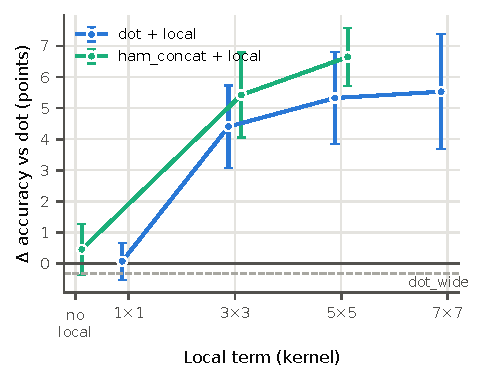
\includegraphics[width=\anchocolumna]{figuras/kernel.pdf}
  \caption{Accuracy difference against \var{dot} by size of the local term, with and without the \emph{pooling} branch of \var{ham\_concat} (seeds 0--4, 95~\% CI). The dashed line is the capacity control \var{dot\_wide}.}
  \label{fig:kernel}
\end{figure}

% Translated by scripts/tables_en.py from the Spanish table generated by scripts/ieee_tables.py a partir de los runs; no editar a mano.

\begin{table*}[!t]
\centering
\footnotesize
\caption{Ablation of the output terms on CIFAR-10 (seeds 0--4, 400 epochs). Paired differences against \texttt{dot} (80.04 $\pm$ 0.31) and against \texttt{dot\_local} ($3\times3$), with the number of favorable seeds in parentheses.}
\label{tab:ablacion}
\begin{adjustbox}{max width=\linewidth}
\begin{tabular}{lrcccrr}
\toprule
Variant & Params. & Accuracy (\%) & $\Delta$ vs \texttt{dot} & $\Delta$ vs \texttt{dot\_local} & Epoch $\geq$79 & s/epoch \\
\midrule
\texttt{dot\_local\_k1} & 119\,674 & 80.11 $\pm$ 0.31 & $+0.07$ [$-0.52$, $+0.67$] & $-4.33$ [$-5.43$, $-3.24$] (0/5) & 205 & 1.51 \\
\texttt{dot\_local} & 121\,210 & 84.44 $\pm$ 0.85 & $+4.40$ [$+3.08$, $+5.73$] & --- & 69 & 1.47 \\
\texttt{dot\_local\_k5} & 124\,282 & 85.36 $\pm$ 1.16 & $+5.32$ [$+3.84$, $+6.81$] & $+0.92$ [$-0.21$, $+2.05$] (5/5) & 53 & 1.49 \\
\texttt{dot\_local\_k7} & 128\,890 & 85.57 $\pm$ 1.27 & $+5.53$ [$+3.67$, $+7.38$] & $+1.12$ [$-0.24$, $+2.48$] (5/5) & 51 & 1.66 \\
\texttt{dot\_gate} & 128\,698 & 80.16 $\pm$ 0.50 & $+0.12$ [$-0.26$, $+0.51$] & $-4.28$ [$-5.57$, $-3.00$] (0/5) & 193 & 1.44 \\
\texttt{dot\_global} & 124\,298 & 80.17 $\pm$ 0.44 & $+0.13$ [$-0.33$, $+0.58$] & $-4.28$ [$-5.61$, $-2.94$] (0/5) & 199 & 2.14 \\
\texttt{dot\_local\_gate} & 130\,618 & 84.19 $\pm$ 0.22 & $+4.15$ [$+3.68$, $+4.62$] & $-0.26$ [$-1.52$, $+1.01$] (3/5) & 64 & 1.57 \\
\texttt{dot\_local\_global} & 126\,218 & 84.30 $\pm$ 0.21 & $+4.26$ [$+3.66$, $+4.85$] & $-0.15$ [$-1.12$, $+0.82$] (3/5) & 69 & 2.27 \\
\texttt{dot\_wide\_local\_k5} & 133\,982 & 85.65 $\pm$ 1.23 & $+5.61$ [$+4.26$, $+6.96$] & $+1.21$ [$-1.12$, $+3.54$] (4/5) & 61 & 1.52 \\
\texttt{ham\_concat\_local} & 130\,826 & 85.46 $\pm$ 1.32 & $+5.42$ [$+4.06$, $+6.79$] & $+1.02$ [$-1.24$, $+3.27$] (4/5) & 72 & 2.45 \\
\texttt{ham\_concat\_local\_k5} & 133\,898 & 86.68 $\pm$ 0.55 & $+6.64$ [$+5.71$, $+7.58$] & $+2.24$ [$+1.26$, $+3.22$] (5/5) & 50 & 2.46 \\
\bottomrule
\end{tabular}
\end{adjustbox}
\end{table*}


\section{Representative Attention Maps}
\label{sec:sup-mapas}
Fig.~\ref{fig:mapas} shows the CLS rollout of \var{dot} with two seeds, of \var{dot\_local\_k5} and of \var{ham\_concat\_local\_k5}, with the same color scale in each row. At a glance, the differences between variants are of the same order as the differences between two seeds of \var{dot}: in several images seed 1 of \var{dot} departs more from seed 0 than the models with a local term do. That is why the comparison is made quantitatively (Table~\ref{tab:mapas}). All divergences are small, because rollout accumulates the residual connection and produces smooth maps. Even so, the models with a local term have maps that are more reproducible across seeds than \var{dot} (JS of 0.0032--0.0055 versus 0.0062), and their distance to \var{dot} exceeds the between-seed variation of \var{dot} by a factor of 1.2 ($3\times3$) to 1.6 (\var{ham\_concat\_local\_k5}) and that of their own seeds by a factor of 1.8 to 3. In other words, the local term produces maps that differ from those of \var{dot} and are consistent across seeds. In an equivalent analysis of the fusions of the first family, by contrast, the distance of each variant to \var{dot} was of the same order as the variation between its own seeds: their maps were less reproducible, but not systematically different. The maps do not include the mixing done by the convolution (Section~\ref{sec:analisis}), so they only show how the attention part changes.

\begin{figure*}[!t]
  \centering
  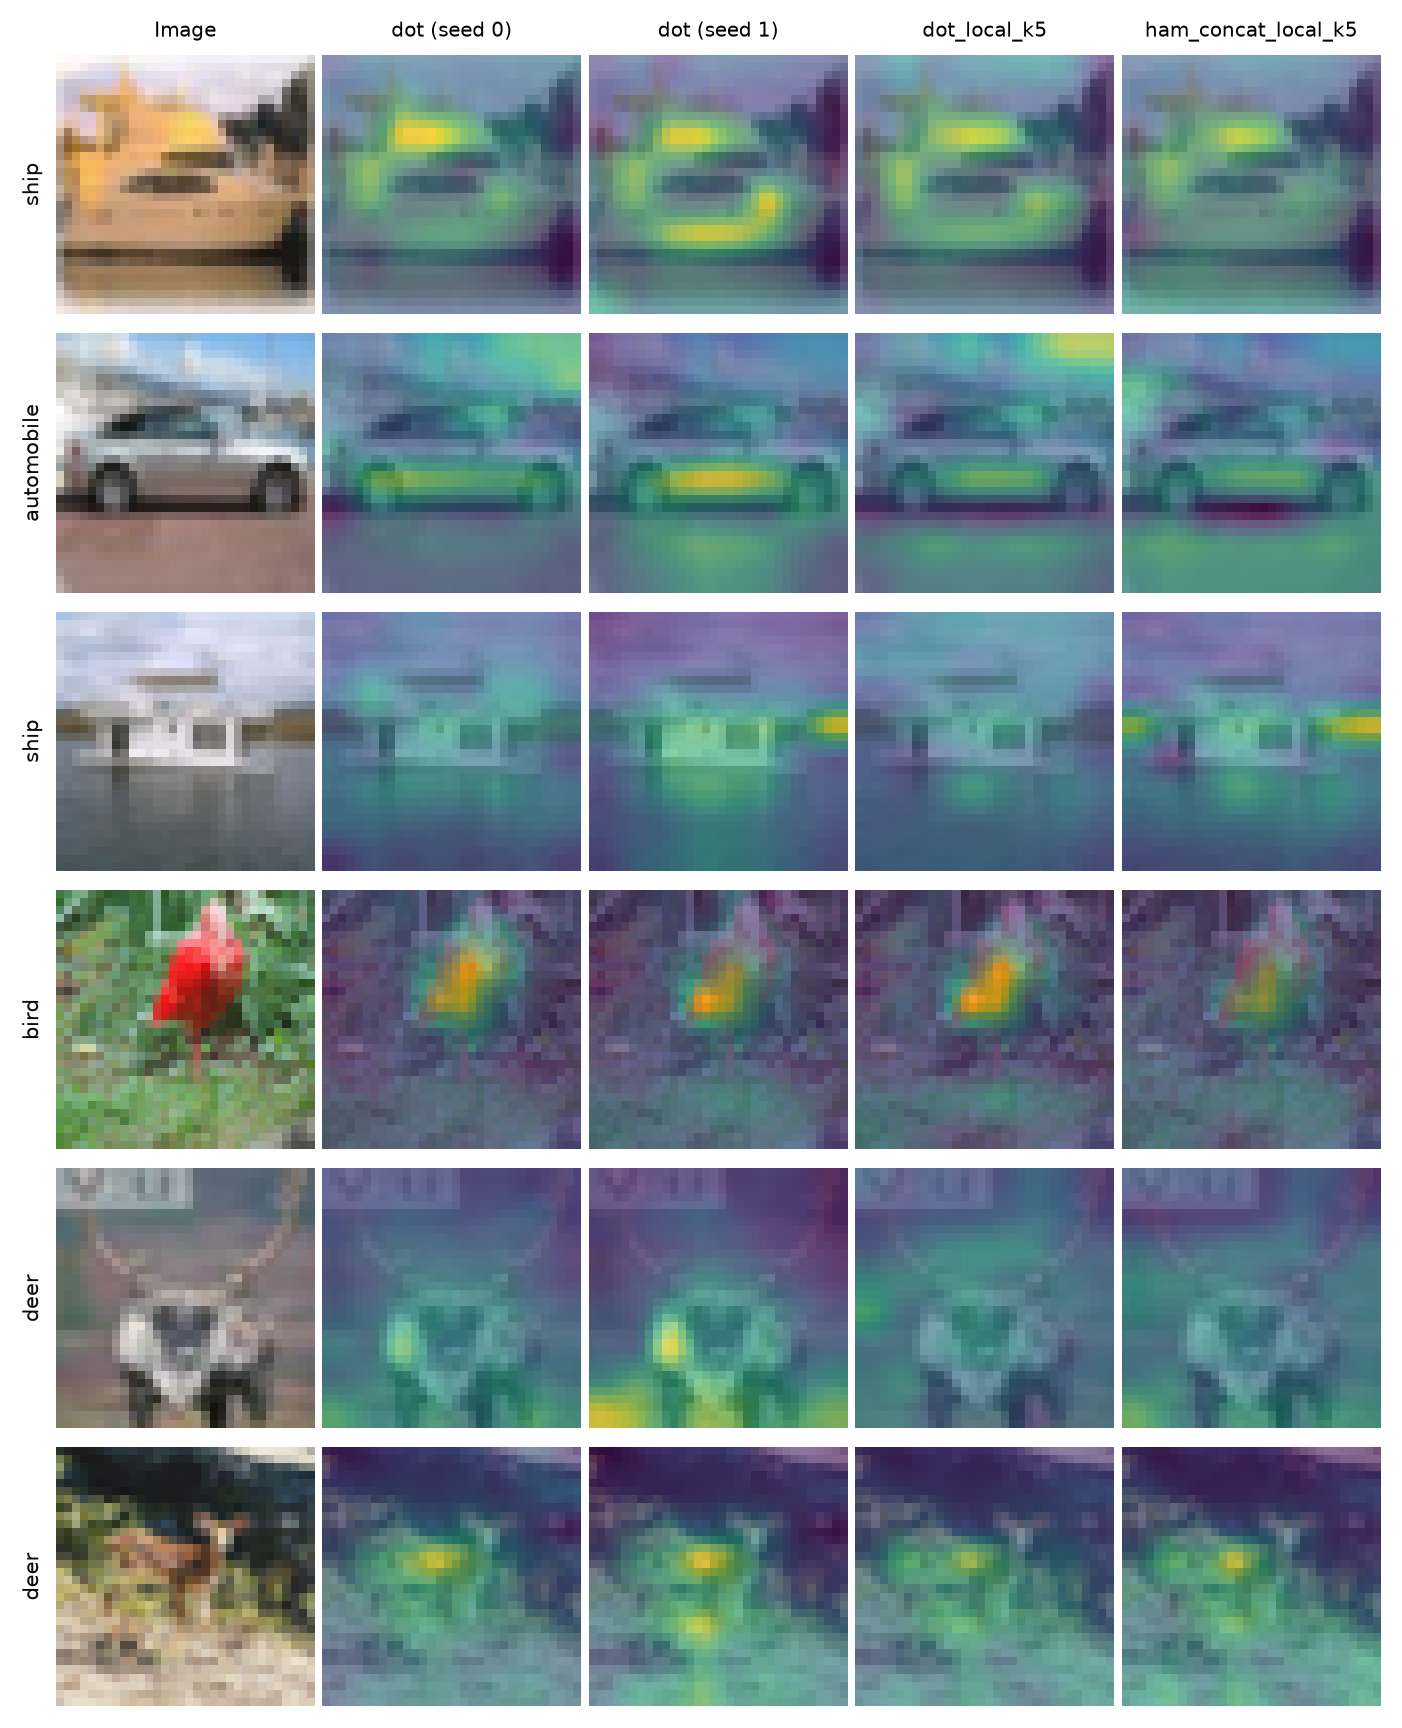
\includegraphics[width=0.62\textwidth]{figuras/mapas.png}
  \caption{CLS \emph{attention rollout} on six CIFAR-10 test images, with a common color scale in each row. The second seed of \var{dot} serves as a control: at a glance, the differences between variants are of the same order as those between two seeds of \var{dot}, so the maps alone do not distinguish the variants; Table~\ref{tab:mapas} compares them against the between-seed variation.}
  \label{fig:mapas}
\end{figure*}

% Translated by scripts/tables_en.py from the Spanish table generated by scripts/paper_tables.py a partir de los runs; no editar a mano.
\begin{table}[tbp]
\centering
\small
\caption{Jensen--Shannon divergence between CLS \emph{rollout} maps on CIFAR-10 (500 test images, seeds 0--4). Between seeds: mean over the 10 seed pairs of the variant. Against \texttt{dot}: same seed. Ratio: against \texttt{dot} divided by the between-seed variation of \texttt{dot}.}
\label{tab:mapas}
\begin{adjustbox}{max width=\columnwidth}
\begin{tabular}{lccc}
\toprule
Variant & JS between seeds & JS against \texttt{dot} & Ratio \\
\midrule
\texttt{dot} & 0.0062 & --- & --- \\
\texttt{dot\_local} & 0.0033 & 0.0076 & 1.22 \\
\texttt{dot\_local\_k5} & 0.0032 & 0.0096 & 1.54 \\
\texttt{ham\_concat\_local\_k5} & 0.0055 & 0.0100 & 1.60 \\
\bottomrule
\end{tabular}
\end{adjustbox}
\end{table}


\section{Sensitivity of the High-Mode Threshold}
\label{sec:sup-umbral}
The threshold of 85.5~\% that separates the two training modes (Section~\ref{sec:res-modos}) was chosen after observing the distribution. Table~\ref{tab:umbral} repeats the counts with thresholds between 85.0 and 86.0~\%. The direction of both comparisons is the same at every threshold: the $5\times5$ term enters the high mode more often than the $3\times3$ term, and the triad more often than its equal-capacity control. Their significance is not: $p$ ranges from 0.023 to 0.083 for $5\times5$ against $3\times3$, and from $<0.001$ to 0.152 for the triad against its control. The second comparison depends on the threshold because the triad also raises the low mode, to about 85~\%: with thresholds of 85.25~\% or lower, part of that mode is counted as high. The frequency comparisons are therefore exploratory, as stated in the main text.

% Translated by scripts/tables_en.py from the Spanish table generated by scripts/ieee_tables.py a partir de los runs; no editar a mano.

\begin{table*}[!t]
\centering
\footnotesize
\caption{Sensitivity of the high-mode frequency to the test-accuracy threshold on CIFAR-10. Seeds in the high mode / seeds; $p$: two-sided Fisher exact test. Left: 16 seeds (0--15); right: the triad and its equal-capacity control with 48 seeds (0--47).}
\label{tab:umbral}
\begin{adjustbox}{max width=\linewidth}
\begin{tabular}{lcccccccc}
\toprule
Threshold (\%) & \texttt{dot\_local} & \texttt{dot\_local\_k5} & \texttt{dot\_wide\_local\_k5} & Triad & $p$ ($5\times5$ vs.\ $3\times3$) & Triad & Control & $p$ \\
\midrule
85.00 & 3/16 & 9/16 & 8/16 & 14/16 & 0.066 & 44/48 & 24/48 & $<0.001$ \\
85.25 & 3/16 & 9/16 & 8/16 & 12/16 & 0.066 & 38/48 & 21/48 & $<0.001$ \\
85.50 (used) & 2/16 & 9/16 & 8/16 & 12/16 & 0.023 & 31/48 & 21/48 & 0.065 \\
85.75 & 2/16 & 9/16 & 8/16 & 11/16 & 0.023 & 29/48 & 21/48 & 0.152 \\
86.00 & 1/16 & 6/16 & 8/16 & 11/16 & 0.083 & 29/48 & 21/48 & 0.152 \\
\bottomrule
\end{tabular}
\end{adjustbox}
\end{table*}



\end{document}
